\documentclass[10pt,a4paper]{article}
\usepackage{fontspec,amsmath,amssymb,amsthm,mathtools,graphicx,bm,bbm,stmaryrd,nicefrac,mathrsfs,braket,xcolor}
\usepackage[margin=22mm]{geometry}
\usepackage[bookmarks=false]{hyperref}
\setlength{\emergencystretch}{3em}
\title{A five-bit seed for perfectly one-private multiparty AND without helpers}
\author{Samuel Dittmer, Rafail Ostrovsky}
\date{doi:10.4230/LIPIcs.ICALP.2026.79; CC BY 4.0}
\begin{document}
\maketitle
\noindent\textit{Editorial note.} Editable TeX converted from the official CC BY HTML prose and math alttext. Original official PDF/HTML retained. Only the specified claim counts; all author context and available source-local supporting proofs are included. Theorem1.5 is the five-bit specialization of general Theorem1.6 and is not an additional collected claim. Corollary1.2 is not counted separately.\par\medskip
\noindent\textit{Editorial note.} Rendering only: four bold Greek Pi protocol labels use boldsymbol rather than mathbf, preserving the original HTML MathML bold Pi and avoiding XeTeX text-font U+0005 remapping.\par\medskip


\par\medskip\noindent\textbf{
1 Introduction}\par




We consider a concrete question in information-theoretic cryptography: How many bits of randomness are required for $n$ parties to compute a Boolean circuit $C$ on their inputs in a $1$-private protocol with semi-honest security?\par




We are motivated by one practical and one theoretical topic of interest in computer science. On the practical side, reducing randomness complexity can improve the usability of cryptographic protocols. In real-world cryptography, random bits must either be collected from physical sources or generated from a pseudo-random number generator applied to some initial seed. There are costs and security risks associated with both approaches, see e.g. [9, 10] and the discussion in [7].\par




On the theoretical side, there is a noteworthy connection between the complexity of $1$-private computation and circuit complexity. As Kushilevitz, Ostrovsky, and Rosén showed [14], any Boolean function $f$ that requires $\omega(1)$ bits of randomness to securely compute requires a circuit of size $\omega(n)$. Therefore, $1$-private randomness complexity of Boolean functions implies circuit lower bounds. Extensions to $t$-privacy were considered in [1, 2].
We study two protocol settings and isolate one combinatorial object that drives the second construction:\par




\begin{itemize}


\item[] 
$\blacksquare$ 


\textbf{Helper-party model:} We allow additional parties that do not have any inputs to assist in the computation [7]. The idea is that one helper party flips a small, truly random seed (here, only two global random bits suffice) and privately distributes the derived one-time bits to the remaining helpers and input parties. The helper parties are then used as “one-time gadgets” for gates. A key point is that each gadget is used only once, so it suffices that \emph{each individual gadget transcript} is statistically (in fact, perfectly) independent of the true secrets when at most one party is corrupted.\par





\item[] 
$\blacksquare$ 


\textbf{No-helper model (AND only):} We remove all helper parties and instead focus on $n$-party AND where each player has an input bit [14, 12, 13, 3]. Again, we want to reuse a tiny seed, but now the helper roles must be \emph{emulated} by parties with inputs. Therefore, each party will play several roles in the protocol. That is, every party participates in multiple steps and receives multiple messages across the computation. Therefore, we must assemble masks so that the entire multi-step view of any single party is consistent with fresh masks in each one-party view, even though everything is globally derived from a single $5$-bit seed.\par





\item[] 
$\blacksquare$ 


\textbf{Sliding-Window Independence Generator:} We isolate a combinatorial object that is behind our no-helper protocol. We define a $(k,m)$-SWIG as a linear Sliding-Window Independence Generator with a $k$-bit seed that outputs $m\geq k$ bits for any $m\geq k$. The SWIG construction must guarantee that every consecutive $k$-bit window of the output, with wrap-around, is uniform. Our AND protocol (without helpers) for $n$ parties uses $(5,n-1)$-SWIG.\par





\end{itemize}


We stress that all our definitions and constructions are information-theoretic and do not rely on any (cryptographic or other) assumptions.\par




\par\medskip\noindent\textbf{
1.1 Our Contributions}\par




Let $C$ be a Boolean circuit over the basis $\{\oplus,\wedge\}$ with constants, with $n$ input wires, $k_{\oplus}$ XOR gates, and $k_{\wedge}$ AND gates, after local preprocessing. We allow unbounded fanout. Public constants are wires rather than gates. The symbol $k$ in SWIG statements is unrelated to the gate counts $k_{\oplus}$ and $k_{\wedge}$.\par



% SOURCE-ID S1.Thmtheorem1


\par\medskip\noindent\textbf{
\textbf{Theorem 1.1}\textbf{.}
}\par



\emph{The function computed by $C$ admits a perfectly $1$-private semi-honest protocol in the helper-party model that uses at most $2$ random bits. For the preprocessed circuit, the protocol uses exactly $1+3k_{\oplus}+7k_{\wedge}$ inputless helper parties, including the single randomness dealer.
Moreover, for $n\geq 3$, the $n$-party AND functionality requires at least $2$ random bits even with arbitrarily many inputless helpers. Hence, for every input length $n\geq 3$, the worst-case randomness complexity in the helper-party model is exactly $2$.}\par



% END-SOURCE-ID S1.Thmtheorem1



Theorem 1.1 uses only $O(|C|)$ helper parties. Combining this with the protocol-to-circuit direction of Kushilevitz, Ostrovsky, and Rosén [14, Lemma 3] gives the following helper-party analog of their circuit/protocol equivalence. In the reverse direction, helper parties are counted as additional parties when applying the KOR protocol-to-circuit lemma.\par



% SOURCE-ID S1.Thmtheorem2


\par\medskip\noindent\textbf{
\textbf{Corollary 1.2}\textbf{.}
}\par



\emph{For a Boolean function family $\{f_{n}:\{0,1\}^{n}\to\{0,1\}\}$, the family has Boolean circuits of size $O(n)$ if and only if it has perfectly $1$-private semi-honest helper-party protocols using at most $2$ random bits and $O(n)$ inputless helpers.}\par



% END-SOURCE-ID S1.Thmtheorem2



Our second result is the following:\par




% SOURCE-ID S1.Thmtheorem3


\par\medskip\noindent\textbf{
\textbf{Theorem 1.3}\textbf{.}
}\par



\emph{For every $n\geq 6$, there is a perfectly $1$-private semi-honest protocol with a single $5$-bit random seed (and no helper parties) for $n$-party AND of their individual inputs.}\par



% END-SOURCE-ID S1.Thmtheorem3




We stress that we do not claim optimality in the no-helper $5$ random-seed case; this is an upper bound only.
Our no-helper construction is based on an exact combinatorial property that the reused masks must satisfy, which we believe is of independent interest:\par



% SOURCE-ID S1.Thmtheorem4


\par\medskip\noindent\textbf{
\textbf{Definition 1.4}\textbf{ }($(k,m)$-SWIG)\textbf{.}
}\par



\emph{For all $k,m\in\mathbb{Z}^{+}$ such that $m\geq k$ we define a $(k,m)$-SWIG to be a locally-computable linear map:
$G:\mathbb{F}_{2}^{k}\to\mathbb{F}_{2}^{m}$
satisfying the following condition: Let $S\leftarrow\mathbb{F}_{2}^{k}$ be uniform, and write
$G(S)=(Z_{0},Z_{1},\ldots,Z_{m-1})$
such that for every $j\in\mathbb{Z}_{m}$, the cyclic window
$(Z_{j},Z_{j+1},\ldots,Z_{j+k-1})$
is uniform over $\mathbb{F}_{2}^{k}$ (all indices are taken modulo $m$). Equivalently, for every $j\in\mathbb{Z}_{m}$ and every $\alpha\in\mathbb{F}_{2}^{k}$,}\par


\[\begin{gathered}
\Pr_{S}[(Z_{j},Z_{j+1},\ldots,Z_{j+k-1})=\alpha]=2^{-k}
\end{gathered}\]


\emph{We can also write $G$ by giving explicit vectors $\mathbf{u}_{0},\mathbf{u}_{1},\ldots,\mathbf{u}_{m-1}\in\mathbb{F}_{2}^{k}$ such that
$G(S)_{i}=\langle\mathbf{u}_{i},S\rangle$
for every output coordinate $i$.}\par



% END-SOURCE-ID S1.Thmtheorem4



When the output length $m$ is fixed, as a shorthand, we call $(k,m)$-SWIG a
$k$-SWIG. Thus, a $5$-SWIG is a five-bit seed generator that outputs a string of length $m$ from a $5$-bit seed such that every length-five sliding window with wraparound in this $m$-bit $5$-SWIG output is uniform.\par



% SOURCE-ID S1.Thmtheorem5


\par\medskip\noindent\textbf{
\textbf{Theorem 1.5}\textbf{ }($5$-SWIG of every output length)\textbf{.}
}\par



\emph{For every $m\geq 5$, there is a $(5,m)$-SWIG over $\mathbb{F}_{2}$.}\par



% END-SOURCE-ID S1.Thmtheorem5



In particular, for every $n\geq 6$, there is a $(5,n-1)$-SWIG over $\mathbb{F}_{2}$. In fact,
we show the following stronger version, although it is not used in our AND protocol:\par



% SOURCE-ID S1.Thmtheorem6


\par\medskip\noindent\textbf{
\textbf{Theorem 1.6}\textbf{ }($k$-SWIG)\textbf{.}
}\par



\emph{For every $k\geq 1$, $m\geq k$, there is an explicit construction of $(k,m)$-SWIG over $\mathbb{F}_{2}$.}\par



% END-SOURCE-ID S1.Thmtheorem6



Our closed-form binary construction of $(k,m)$-SWIGs for every $m\geq k$
can be viewed as an explicit construction of the cyclic-window, fixed-basis
specialization of the classical consecutive-basis interpolation theorem of
Linial and Tarsi [16], and binary
$n$-regular matrix framework of Etzion and Lempel [5].\par




\par\medskip\noindent\textbf{Relation to prior sample-space constructions.}\par




Schulman developed a small sample space local neighborhood
construction [19]. Since cyclic $k$-windows, has neighborhood size $k$ and coordinate degree
$\Delta=k$, Shulman’s construction requires seed length $\lceil k+\log_{2}k\rceil$. Another related work is that of
Kushilevitz and Mansour [11]. In their work,
define $D_{m,k}$ be the maximum number
of distinct nonzero cyclic-window parity tests for a fixed
coordinate. KM sparse-family construction gives seed length
$\lceil\log_{2}(D_{m,k}+1)\rceil$. Moreoever, once $m\geq 2k-1$, the
$D_{m,k}\leq(k+1)2^{k-2}$, becomes equality . Thus,
for $k=5$, KM construction gives $5$ bits for $m=5,6$
and $6$ bits for every $m\geq 7$.\par




$\begin{array}[]{@{}lll@{}}\hline\cr\text{Construction / measure}&\text{general }k&k=5\\
\hline\cr\text{Schulman seed length}&\lceil k+\log_{2}k\rceil&8\text{ bits}\\
\text{Schulman support size}&2^{\lceil k+\log_{2}k\rceil}&256\\
\text{KM sparse seed length}&\lceil\log_{2}(D_{m,k}+1)\rceil&\begin{array}[]{@{}l@{}}5\text{ bits }(m=5,6)\\
6\text{ bits }(m\geq 7)\end{array}\\
\text{KM sparse support size}&2^{\lceil\log_{2}(D_{m,k}+1)\rceil}&\begin{array}[]{@{}l@{}}32\ (m=5,6)\\
64\ (m\geq 7)\end{array}\\
\color[rgb]{0.55,0,0}\definecolor[named]{pgfstrokecolor}{rgb}{0.55,0,0}k\text{-SWIG seed length}&\color[rgb]{0.55,0,0}\definecolor[named]{pgfstrokecolor}{rgb}{0.55,0,0}k&\color[rgb]{0.55,0,0}\definecolor[named]{pgfstrokecolor}{rgb}{0.55,0,0}5\text{ bits}\\
\color[rgb]{0.55,0,0}\definecolor[named]{pgfstrokecolor}{rgb}{0.55,0,0}k\text{-SWIG support size}&\color[rgb]{0.55,0,0}\definecolor[named]{pgfstrokecolor}{rgb}{0.55,0,0}2^{k}&\color[rgb]{0.55,0,0}\definecolor[named]{pgfstrokecolor}{rgb}{0.55,0,0}32\\
\hline\cr\end{array}$\par





\par\medskip\noindent\textbf{SWIG construction optimality for sample spaces.}\par




Define a hypergraph $H$ on $\mathbb{Z}_{m}$ where all cyclic
intervals
$\{i,i+1,\ldots,i+k-1\}$ for $i\in\mathbb{Z}_{m}$ are its hyperedges.
Observe that in this formulation, $k$-SWIG on $m$ bit output is an $H$-wise independent sample space.
Furthermore, $k$-SWIG guarantees that every hyperedge of $H$ is uniform on $\{0,1\}^{k}$
[8]. Equivalently, the $2^{k}\times m$ matrix of
SWIG sliding windows is a cyclic-consecutive test array in which every cyclic
block of $k$ columns contains each $k$-bit word exactly once
[6, 20].
Furthermore, our construction is optimal since any such sample space or test array must have at least
$2^{k}$ rows, as any length-$k$ block must already have $2^{k}$
possible binary patterns. Our SWIG construction achieves this lower bound
with $2^{k}$ rows. Thus, for binary sliding windows,
SWIG gives an explicit optimal construction rather than non-constructive (covering array) bounds of [18, 17].\par





\par\medskip\noindent\textbf{Our SWIG construction is surprisingly simple.}\par




We define $G$ that takes $k$-bit seed $S$, and outputs $m$ bits as follows.
Let $m=qk+s$, where $q\geq 1$ and $0\leq s<k$. We first define vectors $\mathbf{u}_{0},\mathbf{u}_{1},\ldots,\mathbf{u}_{m-1}\in\mathbb{F}_{2}^{k}$ as
$q$ repetitions of
the standard basis vectors $e_{0},\ldots,e_{k-1}$, followed by $\mathbf{b}_{0},\ldots,\mathbf{b}_{s-1}$, (empty if
$s=0$), where $N$ is the least power of two with $N\geq k$, and for
$0\leq t<s$,\par


\[\begin{gathered}
\mathbf{b}_{t}=\left(\binom{N-k}{t},\binom{N-k+1}{t},\ldots,\binom{N-1}{t}\right)\pmod{2}
\end{gathered}\]


where the $i$’th output of $G$ is
$G(S)_{i}=\langle\mathbf{u}_{i},S\rangle$ for each $0\leq i\leq m-1$.\par






\par\medskip\noindent\textbf{
1.2 Preliminaries}\par




Bits are elements of $\mathbb{F}_{2}$, where $a\oplus b=a+b$ and $a\wedge b=ab$.
We use the standard simulation definition for perfect $1$-privacy for semi-honest players. For a protocol $\Pi$, and input vector $\mathbf{a}$, and a party $i$, the view of party $i$ maintains the identities of the senders and receivers to party $i$ and the chronological order of messages to and from party $i$. The view of player $i$ in protocol $\Pi$ is defined as:\par


\[\begin{gathered}
\mathsf{View}_{i}^{\Pi}(\mathbf{a})=(\text{input }a_{i}\text{ (if any)},\ \text{$i$'s random tape},\ \text{all $\Pi$ messages to/from player $i$})
\end{gathered}\]


In our helper-party construction, one distinguished helper party acts as the randomness dealer. It samples two random bits and sends deterministic functions of them over private point-to-point channels.\par



% SOURCE-ID S1.Thmtheorem7


\par\medskip\noindent\textbf{
\textbf{Definition 1.7}\textbf{ }(Perfect 1-privacy)\textbf{.}
}\par



\emph{A protocol $\Pi$ that computes a deterministic functionality $f$ with one public output bit is perfectly $1$-private if the following condition holds. For every party $i$ there is a simulator $\mathsf{Sim}_{i}$. For every input vector $\mathbf{a}$, the real view $\mathsf{View}_{i}^{\Pi}(\mathbf{a})$ has exactly the same distribution as $\mathsf{Sim}_{i}(a_{i},f(\mathbf{a}))$ when $i$ is an input party. It has exactly the same distribution as $\mathsf{Sim}_{i}(f(\mathbf{a}))$ when $i$ is an inputless helper party. The public output broadcast is included in every view.}\par



% END-SOURCE-ID S1.Thmtheorem7



The \emph{randomness complexity} of a protocol counts only fresh random bits, and does not count any bits that are derived from (a combination) of these bits.
We use cyclic indexing for SWIG outputs: when $J$ is an ordered cyclic set of size $m$, $x_{i+t}$ is obtained by advancing $t$ positions in $J$. A cyclic length-$k$ window is the ordered tuple $(x_{i},x_{i+1},\ldots,x_{i+k-1})$. The SWIG condition requires that cyclic windows of length $k$ be uniform. We stress that the SWIG condition does not require ordinary $k$-wise independence among arbitrary subsets of positions.
Since a SWIG is linear and has a $k$-bit seed, Definition 1.4 has a useful equivalent form. For each $j$, the sliding window map\par


\[\begin{gathered}
S\mapsto(Z_{j},Z_{j+1},\ldots,Z_{j+k-1})
\end{gathered}\]


is a linear bijection from $\mathbb{F}_{2}^{k}$ to $\mathbb{F}_{2}^{k}$.
That is, our SWIG is specified by public vectors $\mathbf{u}_{0},\mathbf{u}_{1},\ldots,\mathbf{u}_{m-1}\in\mathbb{F}_{2}^{k}$ and outputs
$Z_{i}=\langle\mathbf{u}_{i},S\rangle$
The following simple rank condition is the one we use in our SWIG construction.\par



% SOURCE-ID S1.Thmtheorem8


\par\medskip\noindent\textbf{
\textbf{Lemma 1.8}\textbf{ }(SWIG rank condition)\textbf{.}
}\par



\emph{Public vectors $\mathbf{u}_{0},\mathbf{u}_{1},\ldots,\mathbf{u}_{m-1}$ is a
$(k,m)$-SWIG if and only if every length $k$ sliding window,
$\mathbf{u}_{j},\mathbf{u}_{j+1},\ldots,\mathbf{u}_{j+k-1},$
has full rank.}\par



% END-SOURCE-ID S1.Thmtheorem8



\par\medskip\noindent\textbf{Proof.}\par




For any starting position $j$, the SWIG map is linear, and for a random seed $S$, the output window is uniformly exactly when this linear map is onto. Since both the domain and
codomain have dimension $k$, being onto is the same as having full rank of $k$.
$\blacktriangleleft$\par



% SOURCE-ID S1.Thmtheorem9


\par\medskip\noindent\textbf{
$\blacktriangleright$ Remark 1.9 (On privacy proofs in this paper).
}\par



\emph{Many gadgets below output masked values rather than public outputs. For such gadgets we prove that for any one corrupted participant, the full local view is simulatable from the participant’s allowed input and the public output. The proofs all follow the same blueprint: we describe the local view and rewrite each message as a deterministic expression in uniform masks. We then use the fact that adding a fixed secret bit to a uniform mask leaves a uniform bit. These are role-level statements. In the helper-party circuit protocol, wire holders may later send deterministic copies or public toggles of the same masked wire. Lemma 3.1 explains why appending these public functions preserves perfect simulation. In the no-helper protocol, a real party can play several roles. The privacy proof, therefore, gives a joint simulator for its entire view.}\par



% END-SOURCE-ID S1.Thmtheorem9






\par\medskip\noindent\textbf{
2 Base Protocols}\par




This section provides constant-party gadgets. Throughout the circuit composition, an intermediate value $w$ is stored as $w+r_{1}$ under a global mask bit $r_{1}$. In the helper-party evaluation of Section 3, the input parties know $r_{1}$. Intermediate wire holders are helpers and do not know this bit.\par




\par\medskip\noindent\textbf{
2.1 Masked Addition with matching masks}\par





\textbf{Protocol Interaction Diagram: Masked Addition with three Helpers $\Pi_{3}$}\par


\par\noindent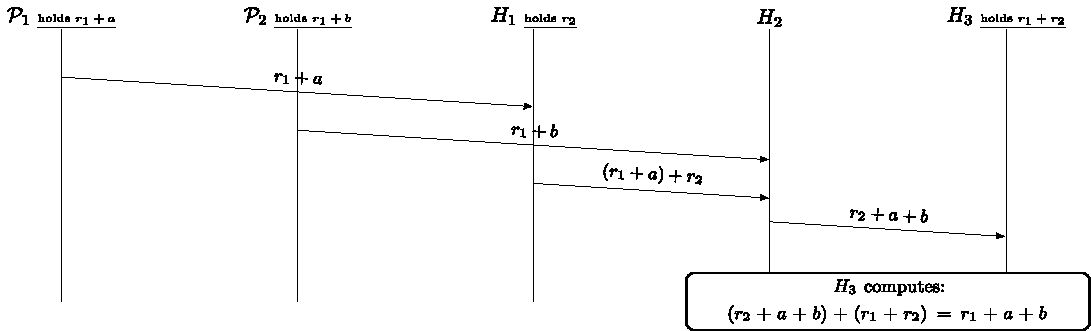
\includegraphics[width=\linewidth,height=0.78\textheight,keepaspectratio]{icalp2026-79-svg-01.pdf}\par





For both $\mathcal{P}_{1}$ and $\mathcal{P}_{2}$, observe that we mask their current input bits by the same random $r_{1}$. Therefore, if the two masked values were added directly, then
$(r_{1}+a)+(r_{1}+b)=a+b$
and masks would cancel each other. This is not useful for our purposes since we need to keep intermediate values hidden.
Therefore, our gadget first temporarily hides the sum under $r_{2}$, then uses $r_{1}+r_{2}$ to convert the result back into the masked value under $r_{1}$. Thus, $H_{2}$ sees only a freshly masked intermediate value.\par





{\bfseries Masked Addition with three Helpers $\boldsymbol{\Pi}_{3}(\mathcal{P}_{1},\mathcal{P}_{2},(H_{i})_{i=1}^{3},a,b,r_{1},r_{2})$


Input.
$\mathcal{P}_{1}$ holds $r_{1}+a$ and $\mathcal{P}_{2}$ holds $r_{1}+b$.
Helpers: $H_{1}$ holds $r_{2}$, $H_{2}$ has no initial input, and $H_{3}$ holds $r_{1}+r_{2}$. 


Output. $H_{3}$ holds $r_{1}+a+b$.


Protocol.}\par


\begin{enumerate}


\item[] 
1. 


$\mathcal{P}_{1}$ sends $r_{1}+a$ to $H_{1}$.\par





\item[] 
2. 


$\mathcal{P}_{2}$ sends $r_{1}+b$ to $H_{2}$.\par





\item[] 
3. 


$H_{1}$ sends $(r_{1}+a)+r_{2}$ to $H_{2}$.\par





\item[] 
4. 


$H_{2}$ sends $(r_{1}+b)+((r_{1}+a)+r_{2})=r_{2}+a+b$ to $H_{3}$.\par





\item[] 
5. 


$H_{3}$ outputs $(r_{2}+a+b)+(r_{1}+r_{2})=r_{1}+a+b$.\par





\end{enumerate}


Figure 1: $\Pi_{3}$: Secure delegated addition when both inputs share the same mask


% SOURCE-ID S2.Thmtheorem1


\par\medskip\noindent\textbf{
\textbf{Lemma 2.1}\textbf{.}
}\par



\emph{For every single corrupted role in the role experiment of Figure 1, the corrupted party’s view is distributed independently of $(a,b)$.}\par



% END-SOURCE-ID S2.Thmtheorem1



\par\medskip\noindent\textbf{Proof.}\par




We check the roles of all five players separately.\par




\emph{The role $\mathcal{P}_{1}$.}
Its view and its message are $r_{1}+a$, which is independent of $a$ since $r_{1}$ is uniform. It is also independent of $b$. The same argument applies to $\mathcal{P}_{2}$, whose only visible bit is $r_{1}+b$.\par




\emph{The role $H_{1}$.}
The view is $(r_{2},r_{1}+a,(r_{1}+a)+r_{2})$. The first two coordinates are independent by the same argument as for $\mathcal{P}_{1}$, and the third is a deterministic function. Thus, the distribution is independent of $(a,b)$.\par




\emph{The role $H_{2}$.}
The two input messages are $r_{1}+b$ and $(r_{1}+a)+r_{2}$ and are independent of
$(a,b)$ for the same reason as above. The outgoing message is their XOR.\par




\emph{The role $H_{3}$.}
$H_{3}$ gets as input $r_{1}+r_{2}$ and $r_{2}+a+b$. This pair of inputs is an invertible affine image of $(r_{1},r_{2})$ for every fixed $(a,b)$. The output is a deterministic function of the pair.\par




Therefore, the simulator for each role can sample the input-independent distributions and append the deterministic outgoing messages.
$\blacktriangleleft$\par






\par\medskip\noindent\textbf{
2.2 Masked Multiplication (one helper, three random bits)}\par




The one-helper multiplication gadget uses three random bits $r_{1},r_{2},r_{3}$. Party $\mathcal{P}_{1}$ sends $a+r_{1}$. Party $\mathcal{P}_{2}$ multiplies it by its input $b$, which results in $ab+br_{1}$. The helper computes the correction from $b+r_{2}$, $r_{1}$, and $r_{1}r_{2}+r_{3}$, since
$r_{1}(b+r_{2})+(r_{1}r_{2}+r_{3})=br_{1}+r_{3}$
$\mathcal{P}_{2}$ adds the correction to $b(a+r_{1})$, which results in $ab+r_{3}$.\par




\textbf{Protocol Interaction Diagram: Masked Multiplication with one helper $\Pi_{1}$ }

\par\noindent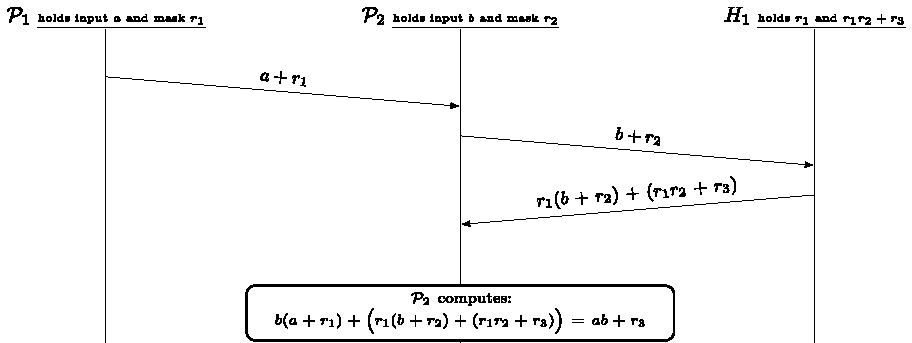
\includegraphics[width=\linewidth,height=0.78\textheight,keepaspectratio]{icalp2026-79-svg-02.pdf}\par
\par





{\bfseries Masked Multiplication with one Helper $\boldsymbol{\Pi}_{1}(\mathcal{P}_{1},\mathcal{P}_{2},H_{1},a,b,r_{1},r_{2},r_{3})$


Input. The first player role receives the masked value $M=a+r_{1}$ (or, in the input-holder variant, knows $(a,r_{1})$ and computes $M$). $\mathcal{P}_{2}$ holds $b$ and $r_{2}$. $H_{1}$ holds $r_{1}$ and $r_{1}r_{2}+r_{3}$.



Output. $\mathcal{P}_{2}$ holds $ab+r_{3}$.


Protocol.}\par


\begin{enumerate}


\item[] 
1. 


$\mathcal{P}_{1}\rightarrow\mathcal{P}_{2}$: send $M=a+r_{1}$.\par





\item[] 
2. 


$\mathcal{P}_{2}\rightarrow H_{1}$: send $b+r_{2}$.\par





\item[] 
3. 


$H_{1}$ sends $r_{1}(b+r_{2})+(r_{1}r_{2}+r_{3})=br_{1}+r_{3}$ to $\mathcal{P}_{2}$.\par





\item[] 
4. 


$\mathcal{P}_{2}$ outputs $b(a+r_{1})+(br_{1}+r_{3})=ab+r_{3}$.\par





\end{enumerate}


Figure 2: $\Pi_{1}$: Secure delegated multiplication with one helper party


% SOURCE-ID S2.Thmtheorem2


\par\medskip\noindent\textbf{
\textbf{Lemma 2.2}\textbf{ }(Privacy for $\Pi_{1}$)\textbf{.}
}\par



\emph{The protocol in Figure 2 is correct and has the following role-level privacy. In the masked-holder variant, the first role sees only $M=a+r_{1}$ and its outgoing copy. Its view is independent of $(a,b)$. In the input-holder variant, the first role’s view is simulatable from $a$ and is independent of $b$. The second role’s view is simulatable from $b$ and is independent of $a$. This remains true even though it outputs the masked value $ab+r_{3}$, whose joint distribution with the rest of the second role’s view remains simulatable from $b$. The helper role’s view is independent of $(a,b)$.}\par



% END-SOURCE-ID S2.Thmtheorem2



\par\medskip\noindent\textbf{Proof.}\par




Correctness follows from
$b(a+r_{1})+\bigl(r_{1}(b+r_{2})+(r_{1}r_{2}+r_{3})\bigr)=ab+r_{3}$
In the masked-holder variant, the first player $\mathcal{P}_{1}$ gets $M=a+r_{1}$, which is independent of $a$.
In the input-holder variant, $\mathcal{P}_{1}$ has $(a,r_{1})$ and sends $a+r_{1}$, where $a$ is his own input.\par




The second role player knows $(b,r_{2})$. It receives $a+r_{1}$, sends $b+r_{2}$, receives $br_{1}+r_{3}$, and outputs $ab+r_{3}$. Conditioned on $(b,r_{2})$, the pair $(a+r_{1},br_{1}+r_{3})$ is an affine image of the uniform pair $(r_{1},r_{3})$. The linear part has matrix $\begin{pmatrix}1&0\\
b&1\end{pmatrix}$ in the variables $(r_{1},r_{3})$ and is invertible. Hence, the pair is independent of $a$. The output is a deterministic function of the same local data, so it is included in the simulated view.\par




The helper roles have $(r_{1},r_{1}r_{2}+r_{3})$, it receives $b+r_{2}$, and sends $r_{1}(b+r_{2})+(r_{1}r_{2}+r_{3})$. For each fixed $b$, observe that the map
$(r_{1},r_{2},r_{3})\longmapsto(r_{1},r_{1}r_{2}+r_{3},b+r_{2})$
is a bijection on $\mathbb{F}_{2}^{3}$. The outgoing message is deterministic and independent of $(a,b)$.
$\blacktriangleleft$\par






\par\medskip\noindent\textbf{
2.3 Masked Multiplication (four helpers, two random bits)}\par





\textbf{Protocol Interaction Diagram: Masked Multiplication with four Helpers $\Pi_{4}$}\par


\par\noindent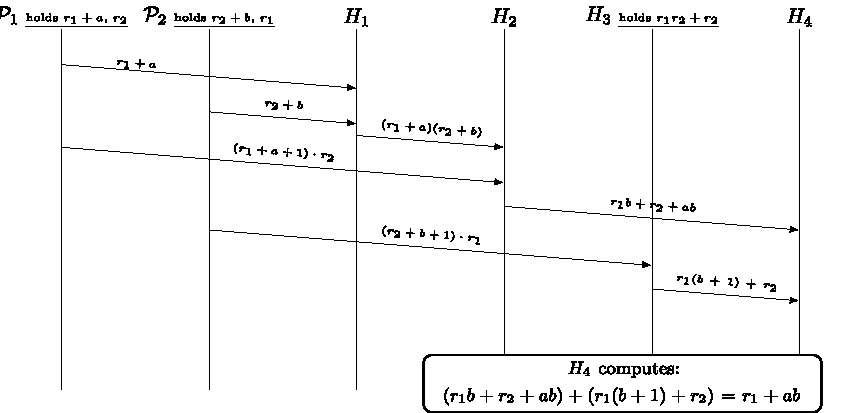
\includegraphics[width=\linewidth,height=0.78\textheight,keepaspectratio]{icalp2026-79-svg-03.pdf}\par





This gadget computes $ab$ while using only the two random bits $r_{1}$ and $r_{2}$. Its output is again masked by $r_{1}$, so it can be used as the input to a later gate.\par




The first helper party $H_{1}$ computes $(r_{1}+a)(r_{2}+b)$. Party $\mathcal{P}_{1}$ computes $(r_{1}+a+1)r_{2}$. Their sum is $r_{1}b+r_{2}+ab$. This follows from $(r_{1}+a)(r_{2}+b)+(r_{1}+a+1)r_{2}=r_{1}b+r_{2}+ab$. Separately, $\mathcal{P}_{2}$ and $H_{3}$ compute $r_{1}(b+1)+r_{2}$. When $H_{4}$ adds these two values, the $r_{2}$ terms cancel, and the final result is $r_{1}+ab$.\par





{\bfseries Masked Multiplication with four Helpers $\boldsymbol{\Pi}_{4}(\mathcal{P}_{1},\mathcal{P}_{2},H^{1},H^{2},H^{3},H^{4},a,b,r_{1},r_{2})$


Input.
$\mathcal{P}_{1}$ holds $r_{1}+a$ and $r_{2}$ and $\mathcal{P}_{2}$ holds $r_{2}+b$ and $r_{1}$.
Helper $H_{3}$ holds $r_{1}r_{2}+r_{2}$. The other helpers receive only the messages specified below.


Output. $H_{4}$ holds $r_{1}+ab$.


Protocol.}\par


\begin{enumerate}


\item[] 
1. 


$\mathcal{P}_{1}\rightarrow H_{1}$: send $r_{1}+a$.\par





\item[] 
2. 


$\mathcal{P}_{2}\rightarrow H_{1}$: send $r_{2}+b$.\par





\item[] 
3. 


$H_{1}\rightarrow H_{2}$: send $(r_{1}+a)(r_{2}+b)$.\par





\item[] 
4. 


$\mathcal{P}_{1}\rightarrow H_{2}$: send $(r_{1}+a+1)\,r_{2}$.\par





\item[] 
5. 


$H_{2}\rightarrow H_{4}$: send $(r_{1}+a)(r_{2}+b)+(r_{1}+a+1)r_{2}=r_{1}b+r_{2}+ab$.\par





\item[] 
6. 


$\mathcal{P}_{2}\rightarrow H_{3}$: send $(r_{2}+b+1)\,r_{1}$.\par





\item[] 
7. 


$H_{3}\rightarrow H_{4}$: send $(r_{2}+b+1)r_{1}+(r_{1}r_{2}+r_{2})=r_{1}(b+1)+r_{2}$.\par





\item[] 
8. 


$H_{4}$ outputs $(r_{1}b+r_{2}+ab)+(r_{1}(b+1)+r_{2})=r_{1}+ab$.\par





\end{enumerate}


Figure 3: $\Pi_{4}$: Secure delegated multiplication with two random bits (with 4 helpers)


% SOURCE-ID S2.Thmtheorem3


\par\medskip\noindent\textbf{
\textbf{Lemma 2.3}\textbf{.}
}\par



\emph{For every player role in Figure 3, its view is distributed independently of $(a,b)$.}\par



% END-SOURCE-ID S2.Thmtheorem3



\par\medskip\noindent\textbf{Proof.}\par




Let $(a,b)$ be two inputs to the multiplication protocol and $r_{1},r_{2}$ to be the two uniform random bits. We show that for every player role, the messages that it sends and receives are independent of $(a,b)$.
Specifically, $P_{1}$ view is
$(r_{2},U,(U+1)r_{2})$ where $U=r_{1}+a$, which is independent of $(a,b)$.
As in the previous proof, the pair $(r_{2},U)$ is uniform, and the last coordinate is a deterministic function of the first two arguments. The argument for $P_{2}$ is the same. If $V=r_{2}+b$, then its view
$(r_{1},V,(V+1)r_{1})$
is uniform over its first two coordinates, with the third determined by the first two.
For $H_{1}$, the received values are $r_{1}+a$ and $r_{2}+b$. This is just an affine translation of random bits, so it is uniform. For $H_{2}$ let
$U=(r_{1}+a)(r_{2}+b)$, and $V=(r_{1}+a+1)r_{2}$
$H_{2}$ view is $(U,V,U+V)$. Enumerating over all four choices for the two random bits gives
$\Pr[(U,V,U+V)=(0,0,0)]=\frac{1}{2},$
and probability $\frac{1}{4}$ for
$(0,1,1)$ and $(1,0,1)$ and no other possible triples with positive probability. Observe that this is again independent of $(a,b)$.\par




For $H_{3}$, set
$L=r_{1}r_{2}+r_{2}$, $I=(r_{2}+b+1)r_{1}$, and $O=L+I$. With this notation,
the view of $H_{3}$ is $(L,I,O)$. It contains no occurrence of $a$, and for both choices of $b$ has exactly the same distribution as for $H_{2}$.\par




Finally, $H_{4}$ receives
$U=r_{1}b+r_{2}+ab$, and $V=r_{1}(b+1)+r_{2}$.
When $b=0$, this becomes
$(U,V)=(r_{2},r_{1}+r_{2}),$
and when $b=1$, it becomes
$(U,V)=(r_{1}+r_{2}+a,r_{2}).$
In both cases, the pair is uniform.
Thus, every single role has a view whose distribution is independent of the inputs $(a,b)$.
$\blacktriangleleft$\par






\par\medskip\noindent\textbf{
2.4 Masked Multiplication with matching masks (seven helpers)}\par





\textbf{Protocol Interaction Diagram: Masked Multiplication with seven Helpers $\Pi_{7}$}\par


\par\noindent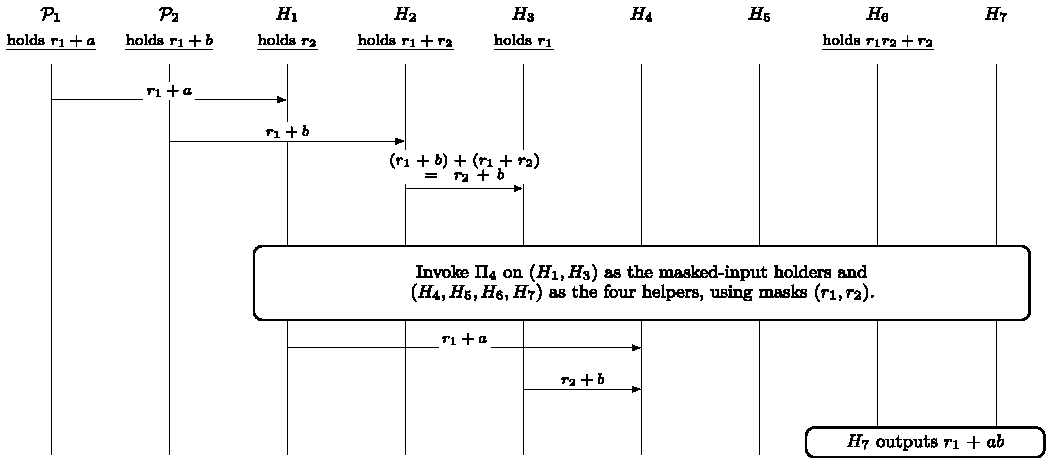
\includegraphics[width=\linewidth,height=0.78\textheight,keepaspectratio]{icalp2026-79-svg-04.pdf}\par





Notice that we start with both inputs being masked by the same $r_{1}$. In the overall circuit protocol, this wrapper is invoked only in the distinct helper mode, separate from the above preprocessing. The $\Pi_{4}$ protocol needs the second input to be masked by $r_{2}$. Therefore, we first convert $r_{1}+b$ into $r_{2}+b$. Helper $H_{2}$ holds $r_{1}+r_{2}$ and can compute $(r_{1}+b)+(r_{1}+r_{2})=r_{2}+b$. The parties then invoke $\Pi_{4}$ on the pair $r_{1}+a$ and $r_{2}+b$. We stress that $\Pi_{7}$ does not
generate any new randomness.\par





{\bfseries Masked Multiplication with seven Helpers $\boldsymbol{\Pi}_{7}(\mathcal{P}_{1},\mathcal{P}_{2},H^{1},\ldots,H^{7},a,b,r_{1},r_{2})$


Input.
$\mathcal{P}_{1}$ holds $r_{1}+a$ and $\mathcal{P}_{2}$ holds $r_{1}+b$.
Helpers: $H_{1}$ has $r_{2}$, $H_{2}$ has $r_{1}+r_{2}$, $H_{3}$ has $r_{1}$, and $H_{6}$ has $r_{1}r_{2}+r_{2}$.


Output. $H_{7}$ gets $r_{1}+ab$.


Protocol.}\par


\begin{enumerate}


\item[] 
1. 


$\mathcal{P}_{1}\rightarrow H_{1}$: send $r_{1}+a$.\par





\item[] 
2. 


$\mathcal{P}_{2}\rightarrow H_{2}$: send $r_{1}+b$.\par





\item[] 
3. 


$H_{2}\rightarrow H_{3}$: send $(r_{1}+b)+(r_{1}+r_{2})=r_{2}+b$.\par





\item[] 
4. 


Call\par


\[\begin{gathered}
\Pi_{4}\bigl(H_{1},H_{3},H_{4},H_{5},H_{6},H_{7},a,b,r_{1},r_{2}\bigr)
\end{gathered}\]


using masks $r_{1},r_{2}$ with (blinded) inputs $a$ and $b$. In $\Pi_{4}$, $H_{1}$ plays the role of $\mathcal{P}_{1}$ with $(r_{1}+a,r_{2})$ and $H_{3}$ plays the role of $\mathcal{P}_{2}$ with inputs $(r_{2}+b,r_{1})$. $H_{6}$ serves as provider of $r_{1}r_{2}+r_{2}$. Finally, $H_{7}$ receives the output.\par





\end{enumerate}


Figure 4: $\Pi_{7}$: Multiplication with two random bits


% SOURCE-ID S2.Thmtheorem4


\par\medskip\noindent\textbf{
\textbf{Lemma 2.4}\textbf{.}
}\par



\emph{For every player role in Figure 4, the party’s view is independent of $(a,b)$.}\par



% END-SOURCE-ID S2.Thmtheorem4



\par\medskip\noindent\textbf{Proof.}\par




$\mathcal{P}_{1}$’s local view consists only of the sent masked value $r_{1}+a$. Similarly, $\mathcal{P}_{2}$’s local view consists of the masked value $r_{1}+b$. Helper $H_{2}$ holds $r_{1}+r_{2}$, receives $r_{1}+b$, and sends $r_{2}+b$ to $H_{3}$. Its view is $(r_{1}+b,r_{1}+r_{2},r_{2}+b)$, where the third coordinate is a deterministic function of the first two coordinates. The first two coordinates are uniform. Thus, every prefix view is independent of $(a,b)$.\par




For parties that appear only in $\Pi_{4}$ call, Lemma 2.3 applies. The only roles that appear both before and during the internal call of $\Pi_{4}$ are $H_{1}$ and $H_{3}$. For $H_{1}$, its view is the first masked-input role of $\Pi_{4}$ with local data $(r_{1}+a,r_{2})$. $H_{1}$ also gets $r_{1}+a$ from $\mathcal{P}_{1}$ before the internal call. $H_{3}$, view is the second masked-input role of $\Pi_{4}$ with local data $(r_{2}+b,r_{1})$. It also sees $r_{2}+b$ received from $H_{2}$ before the internal call. Appending deterministic copies cannot change the distribution. Therefore, every single-party view in $\Pi_{7}$ is independent of $(a,b)$.
$\blacktriangleleft$\par







\par\medskip\noindent\textbf{
3 1-Private computation with helper parties}\par




The construction below (with $1$-privacy) collapses the randomness of arbitrary Boolean circuits to the optimal value of two bits, at the cost of $O(|C|)$ one-time helpers that do not have any inputs themselves. This is orthogonal to the higher-threshold $t>1$ collusion studied by Goyal, Ishai and Song [7].\par




We evaluate the circuit gate by gate, where for every original wire value $w$, we will have a helper party holding it as a masked value $r_{1}+x_{w}$, with the same masked bit $r_{1}$. This immediately creates a problem for the XOR gate, as direct addition would remove this mask. Instead, our protocol uses $\Pi_{3}$ to “remask” the sum. For the AND gate, our protocol uses $\Pi_{7}$. We note that all helper randomness used by these protocols is a deterministic function of the same two random bits $(r_{1},r_{2})$ produced by the dealer. Specifically, the dealer (without any inputs of his own) picks two random bits and distributes the protocol-specific functions of these two bits to other players. Each gate of the original circuit is assigned a constant number of fresh helper parties to evaluate each gate. That is why local independence, while recycling the same randomness, is composable.\par




\par\medskip\noindent\textbf{
3.1 Secure Protocol with Helper Parties}\par




We convert circuits to $\{\oplus,\wedge\}$ basis with public constants. Before the protocol starts, every wire value is represented as $(w,\tau)$ where $\tau$ is a public “switch” command, so that the actual wire value is $w+\tau$. In other words, when $\tau=0$, it is the original value $w$ of the wire. The negation gate is implicitly represented as $\tau=1$, so that when the wire value is computed, it is publicly negated.
Every remaining binary gate has two distinct input wires and two distinct current holders for these input wires.\par




Only the dealer tosses two random bits and sends the resulting combination to each party, as prescribed by the protocol. The remaining parties are deterministic. The protocol evaluates the circuit in topological order, using $\Pi_{3}$ for XOR gates and $\Pi_{7}$ for AND gates. At the end of the protocol, an input-party holder unmasks directly. If the final holder is a helper, it sends the public toggle of the masked output to $\mathcal{P}_{1}$, who unmasks and broadcasts.\par






{\bfseries Secure helper-assisted computation with two random bits


Parties/Input.
Input parties $\mathcal{P}_{1},\ldots,\mathcal{P}_{n}$
hold private inputs $a_{1},\ldots,a_{n}$.
All operations are in $\mathbb{F}_{2}$ using only XOR and AND gates
For circuit $C$ let $k_{\oplus}$ be the number of XOR gates, and $k_{\wedge}$ be the total number AND gates. Before the protocol begins, we (syntactically) simplify $C$ as follows:
we remove gates where one of the input wires is a fixed constant (using our $\tau$ notation as needed). We also eliminate any gate where the two inputs come from a single input wire.
As a result, every invoked gate has two separate input wires
$(u,\tau_{u}),(v,\tau_{v})$ with $u\neq v$.
We allocate three helper parties $H^{1},H^{2},H^{3}$ for each XOR gate, and seven helper parties $H^{1},\ldots,H^{7}$ for each AND gate. We stress that each gate is allocated entirely new helper parties that are exclusive to that gate. We allocate a separate
dealer party that tosses two random bits and distributes combinations of these two bits to all other parties as needed. Therefore, the total number of helper parties is
$1+3k_{\oplus}+7k_{\wedge}$.}\par




Output. All parties receive circuit output $C(a_{1},\ldots,a_{n})$.\par




Protocol.\par


\begin{enumerate}


\item[] 
1. 


\textbf{Dealer.}
The dealer is the only party that tosses coins in our protocol. Specifically, it uniformly samples $(r_{1},r_{2})$ and sends $r_{1}$ to all
input parties. For XOR gates, recall that there are three helper parties, and the dealer sends
$(r_{2},r_{1}+r_{2})$ to $(H^{1},H^{3})$. Recall that there are seven helper parties for each AND gate, and the dealer sends
$(r_{2},r_{1}+r_{2},r_{1},r_{1}r_{2}+r_{2})$ to $(H^{1},H^{2},H^{3},H^{6})$.\par





\item[] 
2. 


\textbf{Masked wires.}
Recall that we denote by $x_{w}$ the value on wire $w$. Let
$M_{w}=r_{1}+x_{w}$. By $\mathrm{hold}(w)$, we denote the party that holds $M_{w}$.
(Observe that for input wires $w_{i}$,
$\mathrm{hold}(w_{i})=\mathcal{P}_{i}$ and $\mathcal{P}_{i}$ can compute $M_{w_{i}}=r_{1}+a_{i}$.)\par





\item[] 
3. 


\textbf{Gates.}
We will evaluate the gates in topological order, from inputs to outputs. For gate $o$, let
$o=((u,\tau_{u}),(v,\tau_{v}),w,\oplus)$ or
$o=((u,\tau_{u}),(v,\tau_{v}),w,\wedge)$ and let $u\neq v$ be the corresponding input wires for $o$.
The two operand values for this gate are therefore $x_{u}+\tau_{u}$ and $x_{v}+\tau_{v}$.\par




In case of $\oplus$-gate, call
$\Pi_{3}(\mathrm{hold}(u),\mathrm{hold}(v),\mathbf{H}_{o},x_{u}+\tau_{u},x_{v}+\tau_{v},r_{1},r_{2})$ and set
$\mathrm{hold}(w)=H_{o}^{3}$.\par




In case of $\wedge$-gate invoke
$\Pi_{7}(\mathrm{hold}(u),\mathrm{hold}(v),\mathbf{H}_{o},x_{u}+\tau_{u},x_{v}+\tau_{v},r_{1},r_{2})$ and set
$\mathrm{hold}(w)=H_{o}^{7}$.
Observe that in all cases $\mathrm{hold}(w)$ is the value $M_{w}=r_{1}+x_{w}$.\par





\item[] 
4. 


\textbf{Output.}
Let the final operand of the function evaluation be $(w_{f},\tau_{f})$.
If $\mathrm{hold}(w_{f})$ is held by some input party, it sends
$(M_{w_{f}}+\tau_{f})+r_{1}$ to all parties. Otherwise, $\mathrm{hold}(w_{f})$ sends
$M_{w_{f}}+\tau_{f}$ to $\mathcal{P}_{1}$, who sends
$(M_{w_{f}}+\tau_{f})+r_{1}=C(a_{1},\ldots,a_{n})$ to all other parties.\par





\end{enumerate}



Figure 5: Gate by Gate computation with Helpers using two random bits



Each input party $\mathcal{P}_{i}$ has input $a_{i}$ receives a mask $r_{1}$ and on an input wire $w$ it sends on the wire value $M+\tau_{w}=r_{1}+x_{w}+\tau_{w}$
where $\tau_{w}$ is public and indicates whether this particular wire bit should be toggled or not.\par



% SOURCE-ID S3.Thmtheorem1


\par\medskip\noindent\textbf{
\textbf{Lemma 3.1}\textbf{ }(Masked-wire fanout)\textbf{.}
}\par



\emph{For some wire $w_{j}$, assume a party contains a masked value
$M_{j}=r_{1}+x_{w_{j}}$.
This party will only send deterministic functions of $M_{j}$. Therefore, the simulator can simulate these functions perfectly.}\par



% END-SOURCE-ID S3.Thmtheorem1



\par\medskip\noindent\textbf{Proof.}\par




Our simulator already samples the party’s local view, including
$M_{j}$. Later messages are deterministic functions of these values
and the circuit description. Given the output, the final broadcast message is also fixed.
Since adding deterministic values does not change the distribution, the
simulated and real views are identical.
$\blacktriangleleft$\par






\par\medskip\noindent\textbf{
3.2 One random bit is not sufficient – even with Helpers}\par




We consider helper parties without any input as additional communication parties. We use the one-random-bit characterization and normal-form lower bound of Kushilevitz, Ostrovsky, Prouff, Rosén, Thillard, and Vergnaud [13, Theorem 4.7]. The exact consequence needed here is the following:\par



% SOURCE-ID S3.Thmtheorem2


\par\medskip\noindent\textbf{
\textbf{Lemma 3.2}\textbf{ }(KOPRTV one-bit obstruction)\textbf{.}
}\par



\emph{For Boolean input parties, the one-bit normal form of [13, Theorem 4.7] cannot compute $\mathrm{AND}_{n}$ when $n\geq 3$.}\par



% END-SOURCE-ID S3.Thmtheorem2



\par\medskip\noindent\textbf{Proof.}\par




This is the public-output Boolean-domain impossibility from [13, Theorem 4.7].
$\blacktriangleleft$\par




Helper can be modeled as an ordinary party whose input is fixed to $\{\star\}$. Such a party remains in the transcript. It does not contribute any input to the normal form.\par



% SOURCE-ID S3.Thmtheorem3


\par\medskip\noindent\textbf{
\textbf{Lemma 3.3}\textbf{ }(1-bit impossibility via the KOPRTV normal form)\textbf{.}
}\par



\emph{Set $n\geq 3$, $m\geq 0$. We define function $F_{n,m}$ as follows:
$F_{n,m}:\{0,1\}^{n}\times\{\star\}^{m}\to\{0,1\}$ ignores
the last $m$ inputs and computes $AND(a_{1},\ldots,a_{n})$.
Then, it is impossible to compute $F_{n,m}$ with perfect $1$-privacy using
only one random bit.}\par



% END-SOURCE-ID S3.Thmtheorem3




\par\medskip\noindent\textbf{Proof.}\par




Assume, for contradiction, that such a protocol exists. If it uses no random
bit, add one unused uniform random bit. Thus, we may assume that it uses exactly
one random bit.\par




Replace each singleton party by a Boolean dummy party with input
$z_{\ell}\in\{0,1\}$. The dummy party runs the same algorithm as before and
ignores $z_{\ell}$. The functionality also ignores $z_{\ell}$. Hence, we obtain a
one-random-bit protocol for the Boolean function
$g(a_{1},\dots,a_{n},z_{1},\dots,z_{m})=\bigwedge_{i=1}^{n}a_{i}$.\par




Correctness is unchanged. Perfect privacy is unchanged as well: the original
simulators handle the parties holding $a_{i}$, while the simulator for a dummy
party ignores $z_{\ell}$ and uses the old singleton-party simulator.\par




By [13, Theorem 4.7], this Boolean-domain protocol has an equivalent
one-bit normal-form representation for $g$. Now fix $z_{1}=\cdots=z_{m}=0$.
After substituting these fixed values, we
obtain a one-bit normal form for
$g(a_{1},\dots,a_{n},0,\dots,0)=\mathrm{AND}_{n}(a_{1},\dots,a_{n})$.\par




However, Lemma 3.2 says that this is impossible, a contradiction.
$\blacktriangleleft$\par



% SOURCE-ID S3.Thmtheorem4


\par\medskip\noindent\textbf{
\textbf{Corollary 3.4}\textbf{ }(Two random bits are necessary for helper-party AND)\textbf{.}
}\par



\emph{For every $n\geq 3$, any perfectly $1$-private AND function, even with arbitrarily many helper parties without any inputs, must use at least two uniform random bits.}\par



% END-SOURCE-ID S3.Thmtheorem4




\par\medskip\noindent\textbf{Proof.}\par




Let a protocol use $m$ helpers. This $m$ is finite in any finite protocol. Lemma 3.3 rules out protocols with at most one uniform random bit for this fixed $m$. Since $m$ was arbitrary, the claim follows.
$\blacktriangleleft$\par



% SOURCE-ID S3.Thmtheorem5


\par\medskip\noindent\textbf{
$\blacktriangleright$ Remark 3.5.
}\par



\emph{The lower bound is used only to rule out one random bit in the worst case, and the case $n=3$ already suffices.}\par



% END-SOURCE-ID S3.Thmtheorem5





\par\medskip\noindent\textbf{
3.3 Sufficiency of Two Random Bits with Helpers}\par




We now prove our Theorem 1.1.\par




\par\medskip\noindent\textbf{Proof.}\par




For the upper bound, order circuit gates in a fixed topological order, and denote, for circuit $C$, the total number of gates as $k$. Each input is held as $r_{1}+x_{w}$. We prove the correctness by induction on this fixed gate order. Consider a gate with inputs $(u,\tau_{u})$ and $(v,\tau_{v})$. The parties with the input to that gate send $r_{1}+x_{u}+\tau_{u}$ and $r_{1}+x_{v}+\tau_{v}$. For the XOR gate, we execute $\Pi_{3}$, which computes $r_{1}+(x_{u}+\tau_{u}+x_{v}+\tau_{v})$. For the AND gate, we execute $\Pi_{7}$ which computes $r_{1}+((x_{u}+\tau_{u})(x_{v}+\tau_{v}))$. Hence, the invariant holds for every circuit wire. We unmask the final result, which reveals $C(a_{1},\dots,a_{n})$.\par




To show privacy for any party $X$ (without collusion) we show a perfect simulator for the view of $X$.\par




If $X$ is a dealer party, its view consists of $(r_{1},r_{2})$ and deterministic outgoing messages to other parties. Hence, the simulator samples $(r_{1},r_{2})$ and computes the same messages.\par




If $X=\mathcal{P}_{i}$, the simulator is given $(a_{i},C(\mathbf{a}))$. It samples $r_{1}\leftarrow\mathbb{F}_{2}$ and outputs the dealer message $r_{1}$. It outputs deterministic messages prescribed by the protocol.
These messages are determined by $a_{i}$, $r_{1}$, and the public toggle $\tau$ for each outgoing message.\par




When $i=1$ and $\mathcal{P}_{1}$ receives the final masked output, the simulator outputs $r_{1}+C(\mathbf{a})$. For parties other then $\mathcal{P}_{1}$, where $\mathrm{hold}(w_{f})=\mathcal{P}_{i}$, the simulator appends the public broadcast $C(\mathbf{a})$.\par




Now suppose $X$ is a helper party that is not the output holder of its gate. This helper party participates in only a single gate computation. Its randomness is derived from a message from the Dealer. If the gate is an XOR gate, Lemma 2.1 simulates its gadget transcript. If the gate is an AND gate, Lemma 2.4 does the simulation.\par




Now, consider the helper party for gate $o$ that holds the (masked) output of that gate. This helper is $H^{3}$ for an XOR gate and $H^{7}$ for an AND gate. For the computation of messages within each gate, we use simulations from Lemma 2.1 for XOR AND Lemma 2.4 for AND gates. This view includes the masked output $M=r_{1}+x_{w}$. If this gate feeds into multiple other gates, consider fan-out wires one by one. Sometimes these fan-out wires have to be toggled – but this is public information from the circuit description.
Therefore, all fan-out messages for a gate are deterministic values of the output of that gate.\par




Every party also receives the final output of the computation. All of these messages can be simulated. Thus, every helper’s view is simulatable.\par




Furthermore, observe that our construction uses exactly $1+3k_{\oplus}+7k_{\wedge}$ helper parties for any circuit computation together with exactly two bits of seed generated by the dealer party.\par




For the lower bound, use Corollary 3.4. It shows that an $n$-party AND with $n\geq 3$ cannot be computed with at most one uniform random bit, even with helpers. Since we have shown a protocol to compute any function $1$-privately with exactly two random bits, the helper-party randomness complexity is exactly two bits (for every input length $n\geq 3$).
$\blacktriangleleft$\par






\par\medskip\noindent\textbf{
3.4 KOR equivalence even with helpers}\par




Kushilevitz, Ostrovsky, and Rosén [14, 15] showed that any $1$ private protocol for a function $f$ that uses only a constant number of random bits implies that $f$ has a linear-size circuit. In this section, we extend this result to $1$-private protocols even in the presence of helper parties.\par



% SOURCE-ID S3.Thmtheorem6


\par\medskip\noindent\textbf{
\textbf{Lemma 3.6}\textbf{ }(Kushilevitz–Ostrovsky–Rosén protocol-to-circuit reduction)\textbf{.}
}\par



\emph{If there exists a perfectly $1$-private semi-honest protocol over private point-to-point channels for a Boolean function on $N$ bits, where each protocol participant receives as his private input exactly one input bit, and the protocol uses $d$ random bits, then this function has a Boolean circuit of size $2^{O(d)}N$.}\par



% END-SOURCE-ID S3.Thmtheorem6



\par\medskip\noindent\textbf{Proof.}\par




In [14] (also, see the journal version, [15, Lemma 3]), consider a $1$-private protocol, where they encode messages as bits, enumerate over all possible random bit strings, and construct a circuit from the protocol. The stated size bound is $2^{O(d)}N$. Our protocol fits their format exactly. Specifically, dealer messages to parties is communication, not additional randomness, and $d\leq 2$.
$\blacktriangleleft$\par





\par\medskip\noindent\textbf{Proof of Corollary 1.2.}\par




Let’s consider any Boolean function on $n$ input bits. If there exists a circuit (over XOR and AND gates) with $O(n)$ gates, then Theorem 1.1 evaluates these circuits with at most two random bits and $O(n)$ helper parties.\par




Conversely, from the upper bound of our theorem 1.1, we already have a
perfectly $1$-private helper-party protocol using at most two random bits and $m(n)=O(n)$ helper parties without input. Define $g_{n}(x_{1},\dots,x_{n},z_{1},\dots,z_{m(n)})=f_{n}(x_{1},\dots,x_{n})$. Thus, the function $g_{n}$ ignores the dummy inputs $z$. We now turn each helper party (without input) into an ordinary input party with a Boolean dummy input $z_{j}$. This input is ignored by the functionality, by the real protocol, and by the simulator. Perfect privacy is therefore preserved. Hence, $g_{n}$ has a no-helper perfectly $1$-private protocol using at most two random bits. Lemma 3.6 gives circuits for $g_{n}$ of size $2^{O(1)}(n+m(n))=O(n)$. Hardwiring the dummy inputs gives circuits for $f_{n}$ of size $O(n)$.
$\blacktriangleleft$\par







\par\medskip\noindent\textbf{
4 Using a $5$-SWIG without helpers}\par




We now prove Theorem 1.3 from $(5,n-1)$-SWIG. We use the one-helper protocol $\Pi_{1}$, shown in Figure 2, as a building block. Observe that in the no-helper setting, every helper role must be played by an input party. The difficulty is that a real party must participate in multiple roles in this protocol. Nevertheless, every party view must still look as if all masks in all roles of this party use fresh random bits.\par




Let $I_{n}=\{2,3,\dots,n\}$. We use indices in $I_{n}$, where $i+d$ is interpreted with wraparound, so that $i+d$ is treated as $2+((i-2+d)\bmod(n-1))$. We fix players in an arbitrary order and then compute prefixes of multiplication. That is, multiplication of step $i$ assumes that we have already (privately) multiplied numbers up to $i-1$, and party
$\mathcal{P}_{i-1}$ has that previous blinded multiplication result. On the other hand, $\mathcal{P}_{i}$ initially acts as a second party with its own private input $a_{i}$, and the role of the helper party will be played by
$\mathcal{P}_{i-2}$. That is, for a fixed $\mathcal{P}_{i}$ with $i\in I_{n}$, he plays the following three roles: he plays the second input role at step $i$ (with input $a_{i})$, the first input role at step $i+1$ if $i<n$ (for $i=n$ transmitting the final result back to $\mathcal{P}_{1}$), and in a helper role at step $i+2$. We stress that these roles are distinct for $|I_{n}|\geq 5$.\par




This warm-up is only a guide to the mask schedule and is not used as the actual proof. Its correctness follows from the same induction as the full protocol with independent masks.\par





{\bfseries Warm-Up: Sequential Composition (not used in final construction)


Input.
$n$ parties $\mathcal{P}_{1},\dots,\mathcal{P}_{n}$ have private inputs $a_{1},\dots,a_{n}$.


Output. All parties get $\prod_{j=1}^{n}a_{j}$.


Protocol.}\par


\begin{enumerate}


\item[] 
1. 


$\mathcal{P}_{1}$ in addition to his usual role, also acts as a dealer, picking uniform random bits $(r_{1},\dots,r_{n+1})$.\par





\item[] 
2. 


$\mathcal{P}_{1}$ distributes $r_{t-1}$, $r_{t+2}$, and $r_{t+2}r_{t+1}+r_{t+3}$ to $\mathcal{P}_{t}$ for $2\leq t\leq n-2$.\par





\item[] 
3. 


Finally, $\mathcal{P}_{1}$ also sends $r_{n-2}$, $r_{2}$, and $r_{2}r_{1}+r_{3}$ to $\mathcal{P}_{n-1}$. It sends $r_{n-1}$, $r_{3}$, and $r_{3}r_{2}+r_{4}$ to $\mathcal{P}_{n}$.\par





\item[] 
4. 


For $i=2,3,\dots,n$, in increasing order, parties execute:\par


\[\begin{gathered}
\Pi_{1}\!\left(\mathcal{P}_{i-1},\mathcal{P}_{i},\mathcal{P}_{i-2},\prod_{j=1}^{i-1}a_{j},a_{i},r_{i},r_{i-1},r_{i+1}\right)
\end{gathered}\]


By roles, we mean the order of arguments in the $\Pi_{1}$ protocol invocation. That is, when a player is called as the first argument to $\Pi_{1}$, we say that he plays the “first” role, and so on. In our calls to $\Pi_{1}$, the first role player holds a smaller prefix result $(\prod_{j=1}^{i-1}a_{j})+r_{i}$ of the multiplication. For the first invocation, when $i=2$, the first role is just player $\mathcal{P}_{1}$ holding $a_{1}+r_{1}$. The second role uses his own private input $a_{i}$ and mask $r_{i-1}$. The third, helper role uses setup bits $r_{i}$ and $r_{i}r_{i-1}+r_{i+1}$. The very first call to $\Pi+1$ is an input-holder variant of $\Pi_{1}$. The rest of the calls to $\Pi_{1}$ are masked-holder variants of $\Pi_{1}$ for all $i>2$.\par





\item[] 
5. 


Finally, $\mathcal{P}_{n}$ sends $(\prod_{j=1}^{n}a_{j})+r_{n+1}$ to $\mathcal{P}_{1}$.\par





\item[] 
6. 


$\mathcal{P}_{1}$ unmasks the message from $\mathcal{P}_{n}$ using $r_{n+1}$ and sends $\prod_{j=1}^{n}a_{j}$ to all parties.\par





\end{enumerate}


Figure 6: $n$-party AND with $n+1$ bits of randomness (baseline)



The warm-up uses an independent mask for each position in the multiplication chain. The SWIG version keeps the same schedule, but it replaces the independent masks by sliding windows coming from the SWIG generator. Our SWIG schedule replaces the triple $(r_{i},r_{i-1},r_{i+1})$ at step $i$ with $(z_{i},z_{i+2},z_{i+1})$.\par




\par\medskip\noindent\textbf{
4.1 The SWIG schedule}\par




Recall that $I_{n}=\{2,3,\dots,n\}$ which we treat cyclically. We will use
a $(5,n-1)$-SWIG, which provides a generator
$G_{n}:\mathbb{F}_{2}^{5}\to\mathbb{F}_{2}^{I_{n}}$
where we set a seed $S$ to be five random bits and denote
$G_{n}(S)=(z_{i})_{i\in I_{n}}$
Recall that by the $5$-SWIG property, every cyclic block of length five
$(z_{i},\ldots,z_{i+4})$ is uniform, with wrap-around. Now, consider step $i$. This step uses $z_{i}$ to mask the AND-prefix of up to $\mathcal{P}_{i-1}$. Player $\mathcal{P}_{i}$ uses $z_{i+2}$ as the mask for his own input $a_{i}$, and uses $z_{i+1}$ as the output mask. Observe that the output mask at step $i$ is exactly the incoming mask at step $i+1$. The dealer sends the following pair to player $\mathcal{P}_{i}$ of values:
$(z_{i+2},\ \ z_{i+2}z_{i+4}+z_{i+3})$
This pair of random bits has two roles. $\mathcal{P}_{i}$ plays the role of second-party at step $i$ and uses the first bit as his mask. The same pair of bits is also used by $\mathcal{P}_{i}$ as a helper party during step $i+2$, because that later step needs helper-role values
$z_{i+2}$ and
$z_{i+2}z_{i+4}+z_{i+3}$.\par



% SOURCE-ID S4.Thmtheorem1


\par\medskip\noindent\textbf{
\textbf{Definition 4.1}\textbf{ }(Randomness complexity for AND without helpers)\textbf{.}
}\par



\emph{For each $n\geq 2$, let $\beta_{n}$ denote the minimum number of uniform random bits required by any perfectly $1$-private semi-honest no-helper protocol for $n$-party AND, allowing arbitrary communication patterns and arbitrary numbers of rounds.}\par



% END-SOURCE-ID S4.Thmtheorem1


% SOURCE-ID S4.Thmtheorem2


\par\medskip\noindent\textbf{
\textbf{Lemma 4.2}\textbf{.}
}\par



\emph{Let $n\geq 6$. If there is a $(5,n-1)$-SWIG over $\mathbb{F}_{2}$, then the protocol in Figure 7 is correct and perfectly $1$-private. Thus, $\beta_{n}\leq 5$.}\par



% END-SOURCE-ID S4.Thmtheorem2




\par\medskip\noindent\textbf{
4.2 The $5$-bit protocol}\par




The protocol follows the warm-up multiplication chain. All masks are now coordinates of the SWIG output. The proof uses only the exact local uniformity of length-five cyclic windows.\par





{\bfseries Full $n$-party AND Protocol


Input.
$n$ parties $\mathcal{P}_{1},\mathcal{P}_{2},\dots,\mathcal{P}_{n}$ hold bits $a_{1},\dots,a_{n}$. 


Output. $\prod_{1}^{n}a_{i}$.


Protocol.}\par


\begin{enumerate}


\item[] 
1. 


$\mathcal{P}_{1}$ samples $S\leftarrow\mathbb{F}_{2}^{5}$ uniformly and computes the $(5,n-1)$-SWIG: $G_{n}(S)=(z_{i})_{i\in I_{n}}$.\par





\item[] 
2. 


$\mathcal{P}_{1}$ sends to $\mathcal{P}_{2\leq i\leq n}$ the following SWIG bits: $(z_{i+2},\,z_{i+2}z_{i+4}+z_{i+3})$.\par





\item[] 
3. 


For $i=2,3,\dots,n$ in increasing order, parties $(\mathcal{P}_{i-1},\mathcal{P}_{i},\mathcal{P}_{\sigma(i)})$ execute $\Pi_{1}$:\par


\[\begin{gathered}
\Pi_{1}\!\left(\mathcal{P}_{i-1},\mathcal{P}_{i},\mathcal{P}_{\sigma(i)},\prod_{j=1}^{i-1}a_{j},a_{i},z_{i},z_{i+2},z_{i+1}\right)
\end{gathered}\]


For each $\Pi_{1}$ call, $\mathcal{P}_{i-1}$ uses as his input the running product $(\prod_{j=1}^{i-1}a_{j})+z_{i}$. For the very first call to $\Pi_{1}$ with $i=2$, since $\mathcal{P}_{i-1}=\mathcal{P}_{1}$, $\mathcal{P}_{1}$ uses his input-holder variant of $\Pi_{1}$. In the second role of $\Pi_{1}$ invocation, party $\mathcal{P}_{i}$ uses his input $a_{i}$ and mask $z_{i+2}$. The helper role $\mathcal{P}_{i-2}$ uses SWIG bits $z_{i}$ and $z_{i}z_{i+2}+z_{i+1}$.\par





\item[] 
4. 


$\mathcal{P}_{n}$ sends $(\prod_{j=1}^{n}a_{j})+z_{n+1}$ to $\mathcal{P}_{1}$.\par





\item[] 
5. 


Finally, $\mathcal{P}_{1}$ unmasks $\mathcal{P}_{n}$’s with $z_{n+1}$ and then sends the ouput $\prod_{j=1}^{n}a_{j}$ to all other parties.\par





\end{enumerate}


Figure 7: Full $n$-party AND protocol with $5$-bit seed and without helpers.




\par\medskip\noindent\textbf{
4.3 Proof of Lemma 4.2
}\par




We will describe a party’s simulated view by grouping its messages according to
the roles it plays. This is only a notational convenience to make our simulation argument easier to present. In the real protocol,
messages are delivered in public chronological order: the setup messages
come first, and then the calls to $\Pi_{1}$ are executed in increasing order. The time when the sender sends a particular message to the receiver is public and fixed for each player. Therefore, a fixed
role-indexed transcript uniquely defines a chronological transcript as well.\par




The simulator may first sample the messages in the role order that is most
convenient for the privacy argument, and this is what we do below. Before outputting such a view, the simulator
reorders those messages according to chronological order. This reordering operates on a transcript and therefore does not introduce new randomness or change the distribution. Therefore, the role-based transcript and chronological transcript have the same distribution after re-ordering.\par




\par\medskip\noindent\textbf{Proof of Lemma 4.2.}\par




For step $i$, let $h=\sigma(i)=i-2$. $\mathcal{P}_{1}$, in his role as a dealer, sends to
$\mathcal{P}_{h}$ SWIG-derived bits:
$(z_{h+2},\ \ z_{h+2}z_{h+4}+z_{h+3})=(z_{i},\ \ z_{i}z_{i+2}+z_{i+1}).$
that $\mathcal{P}_{h}$ in the role of helper at step $i$ requires.\par




We now prove correctness by induction on prefixes $i\leq n$ of the multiplication chain. For $i=2$, $\mathcal{P}_{1}$
transmits $a_{1}+z_{2}$ to $\mathcal{P}_{2}$. When we execute protocol $\Pi_{1}$, it outputs
$a_{1}a_{2}+z_{3}$. Assume that the protocol is correct by induction up to $i<n$ The
output of $\Pi_{1}$ after step $i$ is held by $\mathcal{P}_{i}$, and it holds
$\left(\prod_{j\leq i}a_{j}\right)+z_{i+1}$.
This is the correct first-role input for step $i+1$. Next application of
$\Pi_{1}$ gives
$\left(\prod_{j\leq i+1}a_{j}\right)+z_{i+2}$.
At the $n$’th step, party $\mathcal{P}_{n}$ sends back the final masked product to
$\mathcal{P}_{1}$. Party $\mathcal{P}_{1}$ unmasks the message from
$\mathcal{P}_{n}$ and sends it to everyone.\par




We now prove (perfect) privacy. Let
$f(\mathbf{a})=\prod_{j=1}^{n}a_{j}$. We start by constructing a (perfect) simulator for $\mathcal{P}_{1}$. On input
$(a_{1},f(\mathbf{a}))$, the simulator samples a seed $S$ consisting of five uniform random bits for $5$-SWIG, and computes the $(5,n-1)$-SWIG output
$G_{n}(S)=(z_{i})_{i\in I_{n}}$. It also outputs $a_{1}$, the SWIG seed $S$, and all dealer messages to other players (derived from SWIG output). It also outputs
$i=2$ message $a_{1}+z_{2}$ to $\mathcal{P}_{2}$. The simulator also outputs the last incoming message from $\mathcal{P}_{n}$ (equal to
$f(\mathbf{a})+z_{n+1}$) and final transmission to all other players with the output $f(\mathbf{a})$ of the computation. This perfectly $\mathcal{P}_{1}$’s view.\par




Fix $i\in I_{n}$. Let
$(s_{0},s_{1},s_{2},s_{3},s_{4})=(z_{i},z_{i+1},z_{i+2},z_{i+3},z_{i+4})$
This is a sliding window of length 5 and hence uniform, since it comes from the $5$-SWIG. For $i<n$, party
$\mathcal{P}_{i}$ has three roles: the second input party at step $i$, the first
input party at step $i+1$, and the helper at step $t=i+2$ (recall that $t$
treated cyclically in $I_{n}$). For $i=n$, the first role message at the next
step is replaced by the final send from $\mathcal{P}_{n}$ to $\mathcal{P}_{1}$.\par




We already specified the simulator for $\mathcal{P}_{1}$. Now, we specify simulators for other players (with $\mathcal{P}_{n}$ treated separately).
Let $p_{i-1}=\prod_{j<i}a_{j}$ and $q=s_{2}s_{4}+s_{3}$.
Suppose first that $i<n$. The simulator samples random bits
$s_{2},q,M,H,X$ independently and uniformly. It records the setup
pair $(s_{2},q)$, the incoming step-$i$ message $M$, the second-role outgoing
message $a_{i}+s_{2}$, the helper reply $H$, the next first-role message
$M^{\prime}=a_{i}M+H$
and the helper-role messages $X$ and
$Y=s_{2}X+q$.\par




The last party, $i=n$, is treated separately because its next first-role message
is replaced by the final send. In this case, the simulator samples bits
$s_{1},s_{2},q,M,X$ independently and uniformly. It records the setup
pair $(s_{2},q)$, the incoming step-$n$ message $M$, and the outgoing
second-role message $a_{n}+s_{2}$. It then sets
$M^{\prime}=f(\mathbf{a})+s_{1}.$
The value of $H$ is forced by the relation $H=a_{n}M+M^{\prime}$. Equivalently, if
$a_{n}=0$ it sets $H=M^{\prime}$, while if $a_{n}=1$ it sets $H=M+M^{\prime}$. It records $H$, the
final send $M^{\prime}$, and the helper-role messages $X$ and $Y=s_{2}X+q$.\par




In all cases, the simulator also appends the function output $f(\mathbf{a})$ message from $\mathcal{P}_{1}$.\par




Since we run the simulation in the role-based view, we can also compare it to the real execution in the role-based view. Now, Fix partial product $p_{i-1}$ and input $a_{i}$. In the real protocol, the two visible messages come from the two mask bits $(s_{0},s_{1})$ as:
$(M,H)=(p_{i-1}+s_{0},\ \ a_{i}s_{0}+s_{1})$
Notice that this is just an affine change of variables. In other words, every choice of $(s_{0},s_{1})$ gives exactly one pair $(M,H)$, and every pair $(M,H)$ comes from exactly one choice of $(s_{0},s_{1})$. Since $(s_{0},s_{1})$ is uniform, $(M,H)$ is uniform as well.\par




Here, by the setup pair we mean the two setup values $(s_{2},q)$. The value $s_{2}$ is one of the setup bits, and $q$ is the derived bit given by $q=s_{2}s_{4}+s_{3}$. Now suppose these two values, $s_{2}$ and $q$, have already been fixed. Even then, $s_{4}$ has not been determined. For either possible value of $s_{4}$, there is exactly one choice of $s_{3}$ that makes the equation $q=s_{2}s_{4}+s_{3}$ true. So fixing $(s_{2},q)$ does not make one value of $s_{4}$ more likely than the other. The bit $s_{4}$ is still uniform.\par




Because $a_{t}$ is fixed, the value $X=a_{t}+s_{4}$ is also uniform. Adding the fixed bit $a_{t}$ only possibly flips $0$ and $1$; it does not change the fact that the value is random. Once $X$ is known, however, the helper’s other message is no longer random. It is determined by the formula $Y=s_{2}X+q$. Thus, the helper role has the same behavior in the simulation as it does in the real protocol: first $X$ is uniformly distributed, and then $Y$ is forced by the already fixed setup values.\par




Finally, the randomness used for $(M,H)$ is independent of this remaining choice of $s_{4}$. So the real second-role and helper-role messages have exactly the same joint distribution as the simulator’s messages. Hence, the real and simulated role-indexed views are identically distributed. Reordering the same messages into chronological order does not change this conclusion, so the chronological views are identically distributed as well.
$\blacktriangleleft$\par







\par\medskip\noindent\textbf{
5 Explicit Construction of $k$-SWIGs}\par




\par\medskip\noindent\textbf{
5.1 Non-constructive proof of SWIG existence}\par




For completeness, we first present a self-contained existence proof. This proof essentially derives the cyclic, fixed-basis specialization of the
interpolation-between-bases theorem of Linial and Tarsi [16]. In
rank-matrix language, the condition is closely related to the binary
$n$-regular matrices of Etzion and Lempel [5].\par




Using the equivalence established in Lemma 1.8, we show that there exists a sequence of $m$ vectors such that every sliding window of length $k$ is linearly independent, treating indices mod $m$. First, note that if $e_{1},\dots,e_{k}$ form a basis for $\mathbb{F}_{2}^{k}$, then $e_{1},\dots,e_{k}$ is a $(k,k)$-SWIG. We show how to convert any $(k,m)$-SWIG, for $m\geq k$, into a $(k,m+1)$-SWIG. This conversion relies on the following:\par



% SOURCE-ID S5.Thmtheorem1


\par\medskip\noindent\textbf{
\textbf{Lemma 5.1}\textbf{.}
}\par



\emph{Let $v_{1},v_{2},\dots v_{2n}$ be vectors in $V=\mathbb{F}_{2}^{n+1}$. For $0\leq i\leq n$, let $S_{i}=\{v_{i+1},v_{i+2},\dots v_{i+n}\}$, and for $0\leq i\leq n-1$, let $T_{i}=\{v_{i+1},v_{i+2},\dots v_{i+n+1}\}$. Suppose that for all $i$, the set $T_{i}$ is linearly independent. Then there exists a vector $w\in V$ such that the sets $S_{i}\cup\{w\}$ are all linearly independent.}\par



% END-SOURCE-ID S5.Thmtheorem1



\par\medskip\noindent\textbf{Proof.}\par




Each $S_{i}$ is a subset of a linearly independent set, and so is itself linearly independent; it consequently generates a hyperplane $H_{i}$. Let $p_{i}$ be the unique nonzero element of $V^{*}$ such that $H_{i}=\ker p_{i}$. Each $S_{i}\cup\{w\}$ is linearly independent iff $w\notin H_{i}$ iff $p_{i}(w)=1$.\par




For $0\leq i\leq n-1$, the set $T_{i}$ is $\{v_{i+1}\}\cup S_{i+1}$. Since $T_{i}$ is linearly independent, $v_{i+1}$ is not generated by $S_{i+1}$. Rephrasing, $v_{i+1}\notin H_{i+1}$, so $p_{i+1}(v_{i+1})=1$, i.e. $p_{j}(v_{j})=1$ for $1\leq j\leq n$.\par




Suppose that $c_{0}p_{0}+c_{1}p_{1}+\dots+c_{n}p_{n}=0$ is a nontrivial relation on the $p_{i}$. Let $c_{\ell}$ be the nonzero coefficient of maximal index; since all $p_{i}\neq 0$, necessarily $\ell>0$. We have $c_{0}p_{0}(v_{\ell})+c_{1}p_{1}(v_{\ell})+\dots+c_{\ell}p_{\ell}(v_{\ell})=0$. Now $p_{\ell}(v_{\ell})=1$, while when $i<\ell$, the vector $v_{\ell}$ is in $S_{i}$, so $p_{i}(v_{\ell})=0$. The relation therefore becomes $c_{\ell}\cdot 1=0$, which is absurd. The $p_{i}$ are therefore linearly independent.\par




Since there are $n+1$ vectors $p_{i}$, they form a basis of $V^{*}$. Setting $\varphi(p_{i})=1$ for all $i$ then defines an element $\varphi\in V^{**}$. The canonical isomorphism $V^{**}\cong V$ implies that there exists a unique $w\in V$ such that $\varphi(p)=p(w)$ for all $p\in V^{*}$. We then have $p_{i}(w)=1$ for all $i$.
$\blacktriangleleft$\par




To prove the induction step, let $v_{1},\dots,v_{m}$ be a $(k,m)$-SWIG. Apply the preceding lemma with $n=k-1$; if $m<2k-2$, then set $v_{m+1},\dots,v_{2k-2}=v_{1},\dots,v_{2k-2-m}$. The sets $T_{i}$ from the lemma are sliding windows of length $k$, and so are linearly independent, by the induction hypothesis. Therefore we can apply the lemma to obtain a vector $w\in V$ such that the sets $\{v_{1},\dots,v_{k-1},w\},\{v_{2},\dots,v_{k-1},w,v_{k}\},\dots,\{w,v_{k},\dots,v_{2k-2}\}$ are linearly independent. Inserting $w$ between $v_{k-1}$ and $v_{k}$ gives a $(k,m+1)$-SWIG.\par




We now prove Theorems 1.5 and 1.6. The construction repeats the standard basis and then attaches the Pascal suffix. We will use the following binomial-coefficient identities in our proof:\par






\par\medskip\noindent\textbf{
5.2 Binomial Coefficient Checks}\par



% SOURCE-ID S5.Thmtheorem2


\par\medskip\noindent\textbf{
\textbf{Lemma 5.2}\textbf{ }(Newton Determinants)\textbf{.}
}\par



\emph{For integer-valued $x,h\geq 0$ and $r\geq 1$:}\par


\[\begin{gathered}
\det\Bigl[\binom{x+\beta}{\alpha}\Bigr]=1
\end{gathered}\]


\emph{and}\par


\[\begin{gathered}
\det\Bigl[\binom{h+\alpha+\beta}{\beta}\Bigr]=1
\end{gathered}\]


\emph{where $\alpha$ and $\beta$ range over $0\leq\alpha,\beta<r$. Over integer matrix entries, both determinants are $1$. Furthermore, even after reducing entries modulo two, they both remain $1$.}\par



% END-SOURCE-ID S5.Thmtheorem2



\par\medskip\noindent\textbf{Proof.}\par




Observe that the first determinant evaluates the Newton basis polynomials $\binom{X}{0},\ldots,\binom{X}{r-1}$ at $x,x+1,\ldots,x+r-1$. The second determinant evaluates the polynomials $\binom{h+X}{0},\ldots,\binom{h+X+r-1}{r-1}$ at $0,1,\ldots,r-1$. In both cases, the leading coefficients cancel the consecutive-point Vandermonde products. Therefore, in both cases, the determinant is $1$.
$\blacktriangleleft$\par



% SOURCE-ID S5.Thmtheorem3


\par\medskip\noindent\textbf{
\textbf{Lemma 5.3}\textbf{ }(Complement identity modulo two)\textbf{.}
}\par



\emph{For any non-negative integer $m$, set $N=2^{m}$. Then, for all non-negative integers $x,y$ below $N$,}\par


\[\begin{gathered}
\binom{N-1-x}{y}\equiv\binom{x+y}{y}\pmod{2}
\end{gathered}\]



% END-SOURCE-ID S5.Thmtheorem3




\par\medskip\noindent\textbf{Proof.}\par




Since $N=2^{m}$, we have $N-1=2^{m}-1$, whose $m$ low-order bits are all $1$. Thus, $N-1-x$ can be obtained by flipping $m$ low-order bits of $x$.
We start by considering the left side of the identity. By Lucas’s theorem, $\binom{N-1-x}{y}$ is odd exactly when every $1$-bit of $y$ also appears as a $1$-bit of $N-1-x$. Since the $1$-bits of $N-1-x$ are exactly where $x$ has $0$-bits among the $m$ low-order positions, this means that $x$ and $y$ have no common $1$-bit in their binary representation.
Consider the right-hand side. By the no-carry condition for binomial coefficients mod two, we know that $\binom{x+y}{y}$ is odd exactly when adding $x$ and $y$ in binary representation produces no carries. This condition holds exactly when $x$ and $y$ in binary representation do not have a common $1$ in any position.
Observe that both sides are odd under exactly the same condition — namely that the binary representations of $x$ and $y$ do not have common $1$’s in the same position. If this condition fails, both sides are even. Hence, the two binomial coefficients are congruent modulo two.
$\blacktriangleleft$\par






\par\medskip\noindent\textbf{
5.3 Pascal suffix construction}\par




To the best of our knowledge, our SWIG construction is the first explicit, closed-form construction for binary cyclic windows. The broader consecutive-basis framework goes back to [16, 5].\par




Fix $k\geq 1$ and $m\geq k$. Write $m=qk+s$, where $q\geq 1$ and $0\leq s<k$. Let $e_{1},\ldots,e_{k}$ be the standard basis of $\mathbb{F}_{2}^{k}$. Let $N$ be the least power of two with $N\geq k$, and set $a=N-k$. If $k\geq 2$, define Pascal suffix vectors by coordinates as follows. For $0\leq t\leq k-2$ and $1\leq c\leq k$,
$(\mathbf{b}_{t})_{c}=\binom{a+c-1}{t}\bmod 2$
For $k=1$, there is no suffix. Let the coefficient vectors $\mathbf{u}_{0},\ldots,\mathbf{u}_{m-1}$ consist of $q$ copies of $e_{1},\ldots,e_{k}$, followed by the first $s$ Pascal suffix vectors ${\mathbf{b}_{0}},{\mathbf{b}_{1}},\ldots,{\mathbf{b}_{s-1}}\in\mathbb{F}^{k}_{2}$. The suffix is empty when $s=0$. We are ready to define the SWIG:
$G_{k,m}(S)_{i}=\langle\mathbf{u}_{i},S\rangle$\par



% SOURCE-ID S5.Thmtheorem4


\par\medskip\noindent\textbf{
\textbf{Theorem 5.4}\textbf{ }(Construction and proof of $k$-SWIG Theorem 1.6)\textbf{.}
}\par



\emph{For every $k\geq 1$ and every $m\geq k$, $G_{k,m}$ is a
$(k,m)$-SWIG.}\par



% END-SOURCE-ID S5.Thmtheorem4



\par\medskip\noindent\textbf{Proof.}\par




By Lemma 1.8, it is sufficient to show that every
block of $k$ consecutive coefficient vectors
${\mathbf{u}_{i}},{\mathbf{u}_{i+1}},\ldots,{\mathbf{u}_{i+k-1\pmod{m}}}$
has rank $k$. If $k=1$, this is immediate.
We now assume $k\geq 2$.\par




Any block contained entirely in the repeated standard-basis part is a basis.
It remains to consider boundary blocks, namely those spilling into or out of the Pascal suffix.
Let $r$ be the number of suffix rows in such a block. Then $1\leq r\leq s$.\par




There are two cases. First, a block may enter the Pascal suffix from the repeated
standard basis part. In this case, after deleting the standard-basis pivot rows, the
remaining $r\times r$ matrix has entries, for $0\leq\alpha,\beta<r$,
$\left[\binom{a+\ell+\beta}{\alpha}\right]$
where $0\leq\ell\leq k-r$. Its determinant is $1$ by
Lemma 5.2.\par




Second, a block may start in the Pascal suffix vectors and wrap around to the standard basis. There is some $0\leq j\leq s-r$, such that the reduced matrix is
$M_{\alpha,\beta}=\binom{N-r+\beta}{j+\alpha}$
for $0\leq\alpha,\beta<r$. Reverse the columns, set $x=r-1-\beta$. The entries therefore become
$\binom{N-1-x}{j+\alpha}$
and since $j+\alpha\leq k-2<N$, Lemma 5.3 gives, modulo
$2$,
$\binom{N-1-x}{j+\alpha}=\binom{x+j+\alpha}{x}.$
The second equality of Lemma 5.2 now applies and shows that all such determinants are $1$.
We have therefore now considered all possible cyclic length-$k$ blocks.
$\blacktriangleleft$\par






\par\medskip\noindent\textbf{
5.4 SWIG construction for $k=5$
}\par




\par\medskip\noindent\textbf{Proof of Theorem 1.5.}\par




We spell out the $(5,m)$-SWIG of Theorem 5.4.\par




For any $m\geq 5$ we first determine $q$ and $s$ where
$m=5q+s$, with $q\geq 1$ and $0\leq s<5$. We let
$e_{1},\ldots,e_{5}$ be standard basis of $\mathbb{F}_{2}^{5}$.
We pick $N$ such that $5\leq N$ and is a power of two. That give $N=8$ and $a=N-5=3$. Following Theorem 5.4 for
$0\leq t\leq 3$, define\par


\[\begin{gathered}
\mathbf{b}_{t}=\left(\binom{a}{t},\binom{a+1}{t},\binom{a+2}{t},\binom{a+3}{t},\binom{a+4}{t}\right)\pmod{2}
\end{gathered}\]


Since $a=3$, the suffix vectors become:\par


\[\begin{gathered}
\mathbf{b}_{t}=\left(\binom{3}{t},\binom{4}{t},\binom{5}{t},\binom{6}{t},\binom{7}{t}\right)\pmod{2}
\end{gathered}\]


Since $t$ goes from $0$ to $3$, the suffix vectors mod 2 become:\par


\[\begin{gathered}
\mathbf{b}_{0}=(1,1,1,1,1)\qquad\mathbf{b}_{1}=(1,0,1,0,1)\qquad\mathbf{b}_{2}=(1,0,0,1,1)\qquad\mathbf{b}_{3}=(1,0,0,0,1)
\end{gathered}\]


We now form the coefficient sequence by starting with $q$ copies of basis vectors
$e_{1},e_{2},e_{3},e_{4},e_{5},$
and finishing with Pascal suffix vectors:
$\mathbf{b}_{0},\ldots,\mathbf{b}_{s-1}$
If $s=0$, we append nothing to the basis vectors. This gives coefficient vectors
$\mathbf{u}_{0},\ldots,\mathbf{u}_{m-1}\in\mathbb{F}_{2}^{5}$. The $5$-SWIG takes 5 random bits as a seed $S$, and the $i$’th bit of $(5,m)$-SWIG is
$G(S)_{i}=\langle\mathbf{u}_{i},S\rangle$.
$\blacktriangleleft$\par







\par\medskip\noindent\textbf{
6 Additional results}\par




\par\medskip\noindent\textbf{
6.1 A limitation of the five-bit cyclic framework for $n=5$
}\par




The next obstruction concerns whether there is a transformation-based formulation beyond SWIG. It is not a limitation of the abstract SWIG definition itself. The SWIG protocol requires output length $m=n-1\geq 5$, so it does not apply to $n=5$. One might still try to keep five seed bits and change the helper assignment. The next definition captures the same transformation-based one-helper-per-step framework with an arbitrary helper permutation.\par




This definition is included to connect the $n=5$ obstruction back to the AND protocol. The SWIG schedule in Section 4 is a generator-level sufficient condition for the protocol in Figure 7. It is not the weakest way to express the linear recycling needed by that protocol. A weaker protocol-specific formulation only asks that, after the helper assignment is chosen, each party’s five relevant mask coordinates are uniform and correctly matched to the calls to $\Pi_{1}$. The next definition formalizes this relaxation.\par




Let $I_{n}=\{2,3,\ldots,n\}$, where indexing $i+1$ in $I_{n}$ is defined with wrap-around.\par



% SOURCE-ID S6.Thmtheorem1


\par\medskip\noindent\textbf{
\textbf{Definition 6.1}\textbf{ }(The $5$-agreeable conditions)\textbf{.}
}\par



\emph{Integer $n\geq 2$ is $5$-agreeable if there exists a permutation $\sigma:I_{n}\to I_{n}$ and invertible linear transformations $T_{i}:\mathbb{F}_{2}^{5}\to\mathbb{F}_{2}^{5}$ such that for every $i\in I_{n}$ the following four conditions simultaneously hold:}\par


\[\begin{gathered}
\displaystyle\textbf{(C1)}\quad T_{i}^{\top}\mathbf{e}_{3}=T_{i+1}^{\top}\mathbf{e}_{1}\qquad\textbf{(C2)}\quad T_{\sigma(i)}^{\top}\mathbf{e}_{2}=T_{i}^{\top}\mathbf{e}_{1} \\
\displaystyle\textbf{(C3)}\quad T_{\sigma(i)}^{\top}\mathbf{e}_{4}=T_{i}^{\top}\mathbf{e}_{2}\qquad\textbf{(C4)}\quad T_{\sigma(i)}^{\top}\mathbf{e}_{5}=T_{i}^{\top}\mathbf{e}_{3}
\end{gathered}\]



% END-SOURCE-ID S6.Thmtheorem1



The protocol interpretation is as follows. Suppose $n$ is $5$-agreeable and let $S\leftarrow\mathbb{F}_{2}^{5}$. A transformation-based version of the protocol in Figure 7 uses $\langle T_{i}^{\top}\mathbf{e}_{1},S\rangle$ as the incoming product mask at step $i$, $\langle T_{i}^{\top}\mathbf{e}_{2},S\rangle$ as the input mask for $a_{i}$, and $\langle T_{i}^{\top}\mathbf{e}_{3},S\rangle$ as the output mask. It uses $\mathcal{P}_{\sigma(i)}$ as the helper at step $i$. Party $\mathcal{P}_{h}$ receives the setup pair
$\left(\langle T_{h}^{\top}\mathbf{e}_{2},S\rangle,\,\langle T_{h}^{\top}\mathbf{e}_{2},S\rangle\langle T_{h}^{\top}\mathbf{e}_{4},S\rangle+\langle T_{h}^{\top}\mathbf{e}_{5},S\rangle\right)$
Condition (C1) enforces consistency of masks required between consecutive steps of our $\Pi_{1}$ protocol. Specifically, the
output mask at step $i$ is the next partial product mask at step $i+1$.
The conditions (C2)–(C4) allow proper handling of helper masks. These conditions ensure that the
setup stored by $\mathcal{P}_{\sigma(i)}$ is precisely the helper masks needed
for the $\Pi_{1}$ call at step $i$.\par




Consider party $\mathcal{P}_{i}$, and let $t=\sigma^{-1}(i)$ be the step in which
$\mathcal{P}_{i}$ plays the helper role. Set
$s_{0}=\langle T_{i}^{\top}\mathbf{e}_{1},S\rangle$,
$s_{1}=\langle T_{i}^{\top}\mathbf{e}_{3},S\rangle$,
$s_{2}=\langle T_{i}^{\top}\mathbf{e}_{2},S\rangle$,
$s_{3}=\langle T_{i}^{\top}\mathbf{e}_{5},S\rangle$,
$s_{4}=\langle T_{i}^{\top}\mathbf{e}_{4},S\rangle$.
Now, observe that since $T_{i}$ is invertible, the tuple
$(s_{0},s_{1},s_{2},s_{3},s_{4})$ preserves full rank and is therefore uniform since $T_{i}$ is invertible.\par




The entries $s_{0},s_{1},s_{2}$ are the incoming product mask, output mask, and input
mask received by $\mathcal{P}_{i}$ at step $i$. Consider step $t$ for the helper party. Then, conditions
(C2)–(C4) identify $s_{2},s_{4},s_{3}$ as conditions on the previous AND-prefix mask, local input mask, and the output
mask required by our $\Pi_{1}$ protocol. Thus, with these conditions, the local view of $\mathcal{P}_{i}$ has the same
form as in Lemma 4.2. Therefore, the same simulator applies, and
$5$-agreeability is sufficient for the same one-helper-per-step AND
construction.
The SWIG schedule used in Section 4 is a special case. If $z_{i}=\langle\mathbf{u}_{i},S\rangle$ and $\sigma(i)=i-2$, define:\par


\[\begin{gathered}
T_{i}^{\top}\mathbf{e}_{1}=\mathbf{u}_{i}\qquad T_{i}^{\top}\mathbf{e}_{2}=\mathbf{u}_{i+2}\qquad T_{i}^{\top}\mathbf{e}_{3}=\mathbf{u}_{i+1}\qquad T_{i}^{\top}\mathbf{e}_{4}=\mathbf{u}_{i+4}\qquad T_{i}^{\top}\mathbf{e}_{5}=\mathbf{u}_{i+3}.
\end{gathered}\]




The SWIG condition gives invertibility of each $T_{i}$. The four identities above allow us to recycle bits of the protocol in Figure 7. Thus, our $5$-agreeability definition relaxes and is more general than the SWIG conditions. $5$-agreeability allows other helper permutations, and it does not require a single cyclic output sequence with all sliding windows to be uniform. Unfortunately, Lemma 6.3 below rules out more than a failed choice of SWIG for $n=5$. It also rules out this broader five-bit one-helper framework for the five-player case.\par




We use the notation and terminology of Definition 6.1. Thus $I_{n}=\{2,\ldots,n\}$ is read cyclically, and the matrices $T_{2},\ldots,T_{n}$ are invertible.\par



% SOURCE-ID S6.Thmtheorem2


\par\medskip\noindent\textbf{
\textbf{Lemma 6.2}\textbf{ }($5$-agreeable conditions on helpers)\textbf{.}
}\par



\emph{Suppose $(\sigma,(T_{2},\ldots,T_{n}))$ satisfies the conditions of Definition 6.1. Then, for every $i\in I_{n}$, the helper $\sigma(i)$ is neither $i$ nor one of its cyclic neighbors. That is,
$\sigma(i)\notin\{i-1,i,i+1\}$
where addition and subtraction are cyclic in $I_{n}$. Moreover, two indices cannot choose each other as helpers:
$\sigma^{2}(i)\neq i$.}\par



% END-SOURCE-ID S6.Thmtheorem2



\par\medskip\noindent\textbf{Proof.}\par




We have to prove four cases: the first three cases are that $\sigma$ cannot pick itself or one of its cyclic neighbors as helpers, and the fourth case is that two indices cannot be helpers to each other. In all four cases, we will contradict the assumption that all $T_{2},\ldots,T_{n}$ must be invertible.\par




The self-helper case $\sigma(i)=i$ is immediate. If this is the case, then (C2) gives $T_{i}^{\top}\mathbf{e}_{2}=T_{i}^{\top}\mathbf{e}_{1}$. Two coordinates of $T_{i}$ would have the same coefficient vector, thus contradicting the invertibility of $T_{i}$,\par




Now suppose $i$ chooses $i-1$ as its helper, making $\sigma(i)=i-1$. From condition (C2), we get $T_{i-1}^{\top}\mathbf{e}_{2}=T_{i}^{\top}\mathbf{e}_{1}$. From condition (C1) at $i-1$, we also get $T_{i-1}^{\top}\mathbf{e}_{3}=T_{i}^{\top}\mathbf{e}_{1}$. Hence $T_{i-1}^{\top}\mathbf{e}_{2}=T_{i-1}^{\top}\mathbf{e}_{3}$, which is again impossible.\par




The next-neighbor case is where $i$ chooses $i+1$ as its helper, so $\sigma(i)=i+1$.
Differently from the previous case, we will use condition (C4) instead of (C2). Specifically, (C4) gives $T_{i+1}^{\top}\mathbf{e}_{5}=T_{i}^{\top}\mathbf{e}_{3}$, while (C1) at $i$ gives $T_{i}^{\top}\mathbf{e}_{3}=T_{i+1}^{\top}\mathbf{e}_{1}$. Therefore $T_{i+1}^{\top}\mathbf{e}_{5}=T_{i+1}^{\top}\mathbf{e}_{1}$. This collision contradicts the invertibility of $T_{i+1}$.\par




It remains to rule out mutual referrals, where both $i$ and $\sigma(i)$ are helpers of each other. That is, $\sigma^{2}(i)=i$. Applying (C3) at $\sigma(i)$ gives $T_{i}^{\top}\mathbf{e}_{4}=T_{\sigma(i)}^{\top}\mathbf{e}_{2}$. Applying (C2) at $i$ gives $T_{\sigma(i)}^{\top}\mathbf{e}_{2}=T_{i}^{\top}\mathbf{e}_{1}$. Thus $T_{i}^{\top}\mathbf{e}_{4}=T_{i}^{\top}\mathbf{e}_{1}$, a contradiction again.\par




Thus, every forbidden helper choice is impossible, as it would violate the invertibility of (at least one of) the matrices $T_{2},\ldots,T_{n}$.
$\blacktriangleleft$\par



% SOURCE-ID S6.Thmtheorem3


\par\medskip\noindent\textbf{
\textbf{Lemma 6.3}\textbf{.}
}\par



\emph{The integer $n=5$ is not $5$-agreeable.}\par



% END-SOURCE-ID S6.Thmtheorem3




\par\medskip\noindent\textbf{Proof.}\par




Consider any index $i\in I_{5}$. Lemma 6.2 forbids four assignments to the helper role $\sigma(i)$. Specifically, it rules out the following helper choices: $i$ itself, the previous cyclic neighbor $i-1$, and the next cyclic neighbor $i+1$ and mutual helpers.\par




Now, observe that since the cycle has only four elements in $I_{5}$, there is only one index left which is not forbidden, namely $i+2$.
We can conclude that for any $i$, there is only one choice left for $\sigma(i)$, namely $\sigma(i)=i+2$. However, this map has order 2: applying it twice returns every index to its starting position in $I_{5}$. Hence, $\sigma^{2}(i)=i$ for every $i\in I_{5}$ which contradicts the last forbidden condition of lemma 6.2.
We conclude that no admissible helper permutation exists for $I_{5}$, and $n=5$ is not $5$-agreeable.
$\blacktriangleleft$\par



% SOURCE-ID S6.Thmtheorem4


\par\medskip\noindent\textbf{
$\blacktriangleright$ Remark 6.4.
}\par



\emph{Lemma 6.3 rules out this specific five-bit one-helper recycling framework for $n=5$, even with an arbitrary helper permutation. It does not prove that $\beta_{5}>5$, and the value of $\beta_{5}$ is still open. Couteau and Rosén give a six-bit no-helper AND protocol for every $n\geq 3$. In particular, we know that $\beta_{5}\leq 6$ [3, Theorem 14].}\par



% END-SOURCE-ID S6.Thmtheorem4





\par\medskip\noindent\textbf{
6.2 Proof of Theorem 1.3
}\par




\par\medskip\noindent\textbf{Proof of Theorem 1.3.}\par




For every $n\geq 6$, Theorem 1.5 gives a $(5,n-1)$-SWIG. Our Lemma 4.2 applies protocol in Figure 7 with helper map $\sigma(i)=i-2$. The resulting protocol is correct, perfectly $1$-private, and uses exactly the five-bit seed sampled by $\mathcal{P}_{1}$. Thus $\beta_{n}\leq 5$ for all $n\geq 6$.
$\blacktriangleleft$\par







\par\medskip\noindent\textbf{References}\par



\begin{itemize}


\item[] 
[1]

Ran Canetti, Eyal Kushilevitz, Rafail Ostrovsky, and Adi Rosén.


Randomness vs. fault-tolerance.


In James E. Burns and Hagit Attiya, editors, \emph{Proceedings of the
Sixteenth Annual ACM Symposium on Principles of Distributed Computing,
Santa Barbara, California, USA, August 21-24, 1997}, pages 35–44. ACM,
1997.


doi:10.1145/259380.259416.





\item[] 
[2]

Ran Canetti, Eyal Kushilevitz, Rafail Ostrovsky, and Adi Rosen.


Randomness versus fault-tolerance.


\emph{Journal of Cryptology}, 13(1):107–142, 2000.


doi:10.1007/s001459910005.





\item[] 
[3]

Geoffroy Couteau and Adi Rosén.


Random sources in private computation.


In Shweta Agrawal and Dongdai Lin, editors, \emph{Advances in
Cryptology - ASIACRYPT 2022 - 28th International Conference on the Theory
and Application of Cryptology and Information Security, Taipei, Taiwan,
December 5-9, 2022, Proceedings, Part I}, volume 13791 of \emph{Lecture
Notes in Computer Science}, pages 443–473. Springer, 2022.


doi:10.1007/978-3-031-22963-3\_15.





\item[] 
[4]

Samuel Dittmer and Rafail Ostrovsky.


1-private n-party AND from 5 random bits.


Cryptology ePrint Archive, Paper 2025/1121, 2025.


URL: https://eprint.iacr.org/2025/1121.





\item[] 
[5]

T. Etzion and A. Lempel.


An efficient algorithm for generating linear transformations in a
shuffle-exchange network.


\emph{SIAM Journal on Computing}, 15(1):216–221, February 1986.


doi:10.1137/0215015.





\item[] 
[6]

Anant P. Godbole, Markos V. Koutras, and Fotios S. Milienos.


Binary consecutive covering arrays.


\emph{Annals of the Institute of Statistical Mathematics},
63(3):559–584, 2011.


doi:10.1007/s10463-009-0240-6.





\item[] 
[7]

Vipul Goyal, Yuval Ishai, and Yifan Song.


Tight bounds on the randomness complexity of secure multiparty
computation.


In Yevgeniy Dodis and Thomas Shrimpton, editors, \emph{Advances in
Cryptology - CRYPTO 2022 - 42nd Annual International Cryptology Conference,
CRYPTO 2022, Santa Barbara, CA, USA, August 15-18, 2022, Proceedings, Part
IV}, volume 13510 of \emph{Lecture Notes in Computer Science}, pages
483–513. Springer, 2022.


doi:10.1007/978-3-031-15985-5\_17.





\item[] 
[8]

Ishay Haviv and Michael Langberg.


$H$-wise Independence.


\emph{Chicago Journal of Theoretical Computer Science}, 2019(3), 2019.


doi:10.4086/cjtcs.2019.003.





\item[] 
[9]

Yuval Ishai, Eyal Kushilevitz, Xin Li, Rafail Ostrovsky, Manoj Prabhakaran,
Amit Sahai, and David Zuckerman.


Robust pseudorandom generators.


In Fedor V. Fomin, Rusins Freivalds, Marta Z. Kwiatkowska, and David
Peleg, editors, \emph{Automata, Languages, and Programming - 40th
International Colloquium, ICALP 2013, Riga, Latvia, July 8-12, 2013,
Proceedings, Part I}, volume 7965 of \emph{Lecture Notes in Computer
Science}, pages 576–588. Springer, 2013.


doi:10.1007/978-3-642-39206-1\_49.





\item[] 
[10]

Yuval Ishai, Amit Sahai, and David A. Wagner.


Private circuits: Securing hardware against probing attacks.


In Dan Boneh, editor, \emph{Advances in Cryptology - CRYPTO 2003,
23rd Annual International Cryptology Conference, Santa Barbara, California,
USA, August 17-21, 2003, Proceedings}, volume 2729 of \emph{Lecture Notes in
Computer Science}, pages 463–481. Springer, 2003.


doi:10.1007/978-3-540-45146-4\_27.





\item[] 
[11]

Eyal Kushilevitz and Yishay Mansour.


Randomness in private computations.


\emph{SIAM J. Discret. Math.}, 10(4):647–661, 1997.


doi:10.1137/S0895480196306130.





\item[] 
[12]

Eyal Kushilevitz, Rafail Ostrovsky, Emmanuel Prouff, Adi Rosén, Adrian
Thillard, and Damien Vergnaud.


Lower and upper bounds on the randomness complexity of private
computations of AND.


In Dennis Hofheinz and Alon Rosen, editors, \emph{Theory of
Cryptography - 17th International Conference, TCC 2019, Nuremberg, Germany,
December 1-5, 2019, Proceedings, Part II}, volume 11892 of \emph{Lecture
Notes in Computer Science}, pages 386–406. Springer, 2019.


doi:10.1007/978-3-030-36033-7\_15.





\item[] 
[13]

Eyal Kushilevitz, Rafail Ostrovsky, Emmanuel Prouff, Adi Rosén, Adrian
Thillard, and Damien Vergnaud.


Lower and upper bounds on the randomness complexity of private
computations of AND.


\emph{SIAM Journal on Discrete Mathematics}, 35(1):465–484, 2021.


doi:10.1137/20M1314197.





\item[] 
[14]

Eyal Kushilevitz, Rafail Ostrovsky, and Adi Rosén.


Characterizing linear size circuits in terms of privacy.


In Gary L. Miller, editor, \emph{Proceedings of the Twenty-Eighth
Annual ACM Symposium on the Theory of Computing, Philadelphia,
Pennsylvania, USA, May 22-24, 1996}, pages 541–550. ACM, 1996.


doi:10.1145/237814.238002.





\item[] 
[15]

Eyal Kushilevitz, Rafail Ostrovsky, and Adi Rosén.


Characterizing linear size circuits in terms of privacy.


\emph{Journal of Computer and System Sciences}, 58(1):129–136, 1999.


doi:10.1006/jcss.1997.1544.





\item[] 
[16]

Nathan Linial and Michael Tarsi.


Interpolation between bases and the shuffle exchange network.


\emph{European Journal of Combinatorics}, 10(1):29–39, 1989.


doi:10.1016/S0195-6698(89)80030-7.





\item[] 
[17]

Lucia Moura, Sebastian Raaphorst, and Brett Stevens.


Upper bounds on the sizes of variable strength covering arrays using
the Lovász local lemma.


\emph{Theoretical Computer Science}, 800:146–154, 2019.


doi:10.1016/j.tcs.2019.10.022.





\item[] 
[18]

Sebastian Raaphorst, Lucia Moura, and Brett Stevens.


Variable strength covering arrays.


\emph{Journal of Combinatorial Designs}, 26(9):417–438, 2018.


doi:10.1002/jcd.21602.





\item[] 
[19]

Leonard J. Schulman.


Sample spaces uniform on neighborhoods.


In \emph{Proceedings of the Twenty-Fourth Annual ACM Symposium on
Theory of Computing}, STOC ’92, pages 17–25. ACM, 1992.


doi:10.1145/129712.129715.





\item[] 
[20]

Ce Shi, Bin Wen, and Jing Lin.


Cyclic consecutive orthogonal arrays.


\emph{Acta Mathematicae Applicatae Sinica (Chinese Series)},
39(5):786–800, 2016.


doi:10.12387/C2016070.





\end{itemize}


\end{document}
